% mnras LaTeX class v3.2 (2023/07/20)
\PassOptionsToPackage{hypertexnames=false}{hyperref}
\documentclass[fleqn,usenatbib]{mnras}

% MNRAS is set in Times font
\usepackage{newtxtext,newtxmath}
\usepackage[T1]{fontenc}

% Allow "van" names to sort correctly in the bibliography
\DeclareRobustCommand{\VAN}[3]{#2}
\let\VANthebibliography\thebibliography
\def\thebibliography{\DeclareRobustCommand{\VAN}[3]{##3}\VANthebibliography}

%%%%% AUTHORS - PACKAGES %%%%%
\usepackage{graphicx}
\usepackage{amsmath}
\usepackage{bm}
\usepackage{bbold}
\usepackage{xcolor}
\usepackage{xspace}
\usepackage{booktabs}
\usepackage{placeins}

% Link / citation / URL colour (override mnras default blue)
\definecolor{mulberry}{RGB}{112, 41, 99}
\hypersetup{
  colorlinks=true,
  linkcolor=mulberry,
  citecolor=mulberry,
  urlcolor=mulberry,
  filecolor=mulberry,
}

%%%%% AUTHORS - COMMANDS %%%%%
% cosmological parameters
\newcommand{\om}{\Omega_\mathrm{m}}
\newcommand{\sig}{\sigma_8}
\newcommand{\h}{h}
\newcommand{\ob}{\Omega_\mathrm{b}}
\newcommand{\ns}{n_\mathrm{8}}
% bias parameters
\newcommand{\bo}{b_1}
\newcommand{\bt}{b_2}
\newcommand{\bs}{b_{s^2}}
\newcommand{\bl}{b_{\Delta}}
% noise parameters
\newcommand{\Ah}{A^\mathrm{noise}_\mathrm{homog}}
\newcommand{\Ao}{A^\mathrm{noise}_{\bo}}
\newcommand{\At}{A^\mathrm{noise}_{\bt}}
\newcommand{\As}{A^\mathrm{noise}_{\bs}}
\newcommand{\Al}{A^\mathrm{noise}_{\bl}}
% stats
\newcommand{\pk}{P_{gg}(k)}
\newcommand{\pgg}{P_{gg}(k)}
\newcommand{\pgm}{P_{gm}(k)}
\newcommand{\bispec}{B_{ggg}(k_1,k_2,k_3)}
\newcommand{\pggsh}{P_{gg}}
\newcommand{\pgmsh}{P_{gm}}
\newcommand{\bispecsh}{B_{ggg}}
\newcommand{\stats}{\pk+\pgm+\bispec}
\newcommand{\kmax}{k_\mathrm{max}}
% units
\newcommand{\hinv}{h^{-1}}
\newcommand{\Gpch}{\hinv\,\mathrm{Gpc}}
\newcommand{\Mpch}{\hinv\,\mathrm{Mpc}}
\newcommand{\hMpc}{h \mathrm{Mpc}^{-1}}
% probability
\newcommand{\post}{p(\theta|x)}
\newcommand{\qpost}{q_\phi(\theta|x)}
% misc
\newcommand{\qq}{\bm{q}}
\newcommand{\nbarlo}{\bar{n} = 1.1 \times 10^{-4} \, (\Mpch)^{-3}}
\newcommand{\nbarfid}{\bar{n} = 2.2 \times 10^{-4} \, (\Mpch)^{-3}}
\newcommand{\nbarhi}{\bar{n} = 5.4 \times 10^{-4} \, (\Mpch)^{-3}}
% names
\newcommand{\mtm}{\texttt{map2map}\xspace}
\newcommand{\mmocks}{\texttt{much\'isimocks}\xspace}
\newcommand{\MMOCKS}{\texttt{MUCH\'ISIMOCKS}\xspace}
\newcommand{\bacco}{BACCO\xspace}
\newcommand{\simbig}{\texttt{SimBIG}\xspace}

% Auto-generated numerical quantities (see paper_quantities.dat header)
\input{paper_quantities.dat}

% comments
\DeclareRobustCommand{\ksf}[1]{{\color{teal}{ksf: #1}}}

%%%%%%%%%%%%%%%%%%% TITLE PAGE %%%%%%%%%%%%%%%%%%%
\title[\mmocks: emulated simulations for SBI]{\mmocks: An emulated cosmological simulation suite for simulation-based inference}

\author[K. Storey-Fisher et al.]{
Kate Storey-Fisher,$^{1,2}$\thanks{E-mail: kstoreyf@stanford.edu}
Ra\'ul Angulo,$^{2,3}$
Marcos Pellejero-Iba\~nez,$^{4}$
and friends \ksf{auth order?}
\\
$^{1}$Kavli Institute for Particle Astrophysics and Cosmology, Stanford University, 452 Lomita Mall, Stanford, CA 94305, USA\\
$^{2}$Donostia International Physics Center, Paseo Manuel de Lardizabal 4, 20018 Donostia-San Sebastian, Spain\\
$^{3}$IKERBASQUE, Basque Foundation for Science, E-48013, Bilbao, Spain\\
$^{4}$Institute for Astronomy, University of Edinburgh, Royal Observatory, Blackford Hill, Edinburgh, EH9 3HJ, UK
}

\date{Accepted XXX. Received YYY; in original form ZZZ}
\pubyear{2026}

\begin{document}
\label{firstpage}
\pagerange{\pageref{firstpage}--\pageref{lastpage}}
\maketitle

\begin{abstract}
Galaxy clustering contains rich cosmological information down to non-linear scales; however, methods to extract this information are currently limited by the high cost of cosmological $N$-body simulations, as well as by the fidelity of galaxy bias modeling.
We use a new approach to generating approximate but robust galaxy mocks: we employ the \mtm full-field emulator to generate particle displacement and velocity fields, and apply the hybrid Lagrangian bias expansion approach to flexibly model biased tracers.
With this forward model, we create a suite of mock 3D galaxy density fields each of size (1 $\Gpch$)$^3$ at $z=0$ spanning 10,000 different cosmologies, called \mmocks; we construct tracer fields with up to 32 bias parameters for cosmology, resulting in a 320,000-mock training set. 
We train a simulation-based inference (SBI) model on summary statistics of the density fields---the galaxy--galaxy power spectrum, the galaxy--matter power spectrum, and the galaxy bispectrum---and infer the cosmological parameters, marginalizing over the bias and noise coefficients.
We validate the pipeline on in-distribution test mocks and find our inferred posteriors to be well-calibrated across the prior range.
With this large suite, we are able to test convergence with the number of simulations: we find that while 20,000 training points are sufficient for the power spectrum, when including the additional statistics precision continues to improve beyond 320,000, and that increasing the number of bias parameter sets per cosmology yields similar constraints as increasing the number of cosmologies.
We also show that we recover unbiased cosmological constraints from an out-of-distribution model, an independent high-resolution $N$-body simulation populated with LRG-like galaxies using extended SubHalo Abundance Matching, demonstrating the generalizability of the approach.
We find that the galaxy--matter power spectrum is critical for breaking parameter degeneracies, and additionally including the bispectrum improves precision, for our LRG-like mock on $\om$ by $\PrecPctShameOodFidPkPgmBVsPkPgmOmegaC\%$, $\sig$ by $\PrecPctShameOodFidPkPgmBVsPkPgmSigmaEight\%$ and $\bo$ by $\PrecPctShameOodFidPkPgmBVsPkPgmBo\%$. \ksf{note: if we use only top model instead of ensemble, it jumps to 39\% for sigma8, which is significantly different. let's discuss using the top-3 ensemble vs just top model}
These results are useful for guiding the design of future SBI approaches for galaxy clustering, and demonstrate a promising approach for full-field inference as well as a range of other potential applications.
The \mmocks suite and the code used in this paper are available at \url{this url}.
\end{abstract}

\begin{keywords}
methods: numerical -- methods: statistical -- galaxies: statistics -- cosmology: large-scale structure of Universe -- cosmological parameters
\end{keywords}

%%%%%%%%%%%%%%%%% BODY OF PAPER %%%%%%%%%%%%%%%%%%

\section{Introduction}

The clustering of galaxies encodes information about the cosmological model describing the universe.
Surveys such as the Sloan Digital Sky Survey \citep{York2000} and most recently the Dark Energy Spectroscopic Instrument \citep{desi_collaboration_validation_2023} have spectroscopically observed millions of galaxies, producing detailed maps of a large volume of the observable universe.
Current and upcoming surveys such as Euclid \citep{collaboration_euclid_2025} and the Roman Observatory \citep{spergel_wide-field_2015,wang_high_2022} will deliver more and more high quality galaxy clustering data sets.

Standard approaches to analyzing this spectroscopic survey data rely on analytic techniques to model summary statistics of the galaxy field , and Monte Carlo techniques to sample the parameters of interest (e.g. \citealt{Alam2017, philcox_boss_2022}).
Analyses are thus largely restricted to two-point statistics on quasi-linear scales, which contain robust cosmological information but do not fully capture the information content in the data.
For instance, the DESI analyses use a perturbation theory approach, and their analysis is limited to $\kmax=0.2$ for the power spectrum and $\kmax=0.12$ for the bispectrum \citep{adame_desi_2025, novell-masot_full-shape_2025}. 
Further, as surveys become more sensitive and statistical uncertainties improve, systematic errors will become increasingly relevant, and the effect of various systematics on clustering statistics---both two-point and higher-order statistics---is difficult to model.

A new approach known as simulation-based inference (SBI), or likelihood-free inference, has shown promise for cosmological inference from galaxy clustering, as it obviates these limitations.
In the SBI approach, only a forward model of the data is required, and the posterior of the input parameters is approximated conditioned on the observed data.
In the case of galaxy clustering, one can thus forward model the full galaxy field and directly measure any statistic, without the need for analytic modeling.
Similarly, one can directly forward model the effects of systematics on the galaxy field, and the statistics simply measured without the need for additional modeling specific to each statistic.
Finally, Monte Carlo methods typically assume a Gaussian form for the likelihood (and must estimate a nontrivial covariance matrix), even though higher-order statistics in particular are known to have non-Gaussian properties \citep{hahn_likelihood_2018}; SBI makes no assumptions about the form of the likelihood.
Further, in the case of galaxy clustering one can learn optimized statistics of the galaxy field for the parameters of interest, effectively using the information in the full galaxy field.

While promising, SBI faces challenges for galaxy clustering analyses.
One key issue is that SBI typically requires many simulations, but cosmological simulations are very computationally expensive.
An $N$-body simulation with the volume and resolution to accurately describe galaxy clustering into the nonlinear regime costs at least hundreds (and up to millions) of CPU hours, and thousands to hundreds of thousands of simulations are generally needed for SBI.
Another challenge is modeling how galaxies populate the dark matter distribution; models must be relatively fast, flexible enough to model various galaxy populations, and accurate down to small scales.

There has been significant recent work that has demonstrated SBI as a promising path forward for the field.
The \simbig collaboration employs a forward model based on the 2,000 $(1 \Gpch)^3$ simulations of the Quijote Latin hypercube \citep{villaescusa-navarro_quijote_2020}; they use the HOD model to populate the simulations with galaxies, choosing 10 HODs per cosmology for a total of 20,000 simulations \citep{hahn_rm_2023-2}.
Using the power spectrum and applying to SDSS BOSS data \citep{Dawson2015}, they achieved constraints on $\sig$ 27\% more precise than the standard analysis thanks to the information in small scales \citep{hahn_rm_2022-1}; subsequent analyses have applied \simbig to the bispectrum \citep{hahn_rm_2023-1}, the marked power spectrum \citep{massara_sc_2024}, and the full galaxy field \citep{lemos_simbig_2023-1, hahn_rm_2023}.
\cite{tucci_eftoflss_2024} generate $10^5$ simulations  based on the effective field theory of large-scale structure (EFTofLSS), and employ neural posterior estimation using the power spectrum and bispectrum out to $\kmax=0.2$; as this model is fully perturbative, they are able to use a Euclid-size volume of 63 $(\Gpch)^3$.
By performing a direct comparison to standard inference, they find that the off-diagonal elements of the covariance matrix are important for constraining $\sig$ accurately, while allowing for a non-Gaussian likelihood is less important.
Using the same forward model, \cite{nguyen_how_2024-1} show that full-field inference yields over a factor of five improvement on the constraint on $\sig$ compared to the power spectrum and bispectrum at the same scale cut of $\kmax=0.12$.
Recent work has also explored forward models based on more complicated and physical models of galaxy formation, albeit at the expense of much smaller volumes.
\cite{santi_robust_2023} employ the 1000-simulation Latin hypercubes of the CAMELS suite \citep{villaescusa-navarro_camels_2021}, which are hydrodynamical simulations with $(25 \Mpch)^3$ volumes, to perform SBI using graph neural networks; they find that their inference on $\om$ is robust to galaxy formation physics.

Given the high computational cost of cosmological simulations are, work has turned to developing emulators that learn the mapping from cosmological parameters to the results of the $N$-body simulation.
Much work has been done on emulators of statistics of the density field, largely for the power spectrum.
Recently, full-field emulators have been developed that output the particle displacement field.
The emulator \mtm \citep{jamieson_field_2023} uses a convolutional neural network-based architecture to map from Zel'dovich approximation displacements to $N$-body displacements, trained on the Quijote simulation suite \citep{villaescusa-navarro_quijote_2020}.
It has been used in a range of applications, such as producing large-volume emulated simulations \citep{scoggins_learning_2025}; variants of \mtm have been designed to emulate modified gravity \citep{saadeh_field-level_2025} and to learn the mapping from non-linear structures to the initial conditions of the universe \citep{doeser_bayesian_2024}.
There has been continued work on developing full-field emulators, with a range of training data and neural architectures \citep{kang_tunes_2026,ullmo_predicting_2026, jacobus_emulating_2026}.

Robustly modeling the galaxy--dark matter connection is a key challenge \citep{wechsler_connection_2018}.
Halo-based models such as the halo occupation distribution (e.g. \citep{peacock_halo_2000-1,Seljak2000,Zheng2005}) populate dark matter halos with galaxies based on halo mass and properties, but their flexibility degrades their robustness, particularly for higher-order statistics (e.g. \citealt{contreras_validating_2024, wang2026}).
More physically motivated models like subhalo-abundance matching (e.g. \citealt{vale_linking_2004,shankar_new_2006, conroy_modeling_2006-1}) are more robust, but require merger trees which are more computationally expensive; even more complicated models like semi-analytic models (e.g. \citealt{somerville_semi-analytic_2008,henriques_galaxy_2015-1,stevens_building_2016, somerville_physical_2015}) and hydrodynamical simulations (e.g. \citep{springel_modeling_2005, vogelsberger_introducing_2014, schaye_eagle_2015}) are both expensive and make specific choices regarding galaxy formation, which makes robustness a challenge.
EFTofLSS offers a perturbative approach that is robust on large scales, but breaks down on small scales \citep{bernardeau_large-scale_2002-1,desjacques_large-scale_2017}.

The hybrid Lagrangian bias expansion (or hybrid effective field theory) offers an approach that is accurate into the small-scale regime while remaining computationally relatively low-cost \citep{modi_simulations_2020, kokron_cosmology_2021,zennaro_bacco_2023}.
It combines the Lagrangian bias expansion, which models the galaxy field as a summation of operators of the dark matter field, with particle displacement and velocity fields from $N$-body simulations to advect them to Eulerian space.
This approach has been shown to be effective down to $k\sim0.6$, and has been used to construct accurate emulators of the power spectrum \citep{pellejero-ibanez_modelling_2022,pellejero-ibanez_bacco_2023}.
\cite{pellejero_ibanez_hybrid-bias_2023} showed that emulated $N$-body displacements with \mtm can be used as inputs to the hybrid bias expansion to provide an accurate model of galaxy abundance.
They found 1-2\% precision on the power spectrum $k\sim0.6$; while there were some biases at intermediate scales, these were absorbed by  nuisance parameters describing stochasticity.
Notably, they found that the robustness held with variations in the cosmological parameters, demonstrating promise for using this approach for cosmological inference.

In this paper, we construct a suite of 3-dimensional mock galaxy fields using our forward model based on the hybrid Lagrangian bias expansion with emulated displacements from the full-field \mtm emulator.
The suite, called \mmocks, consists of both real- and redshift-space mocks at $z=0$ and spans galaxy bias and cosmological parameter space.
This suite opens the door to simulation-based inference for cosmology with a hybrid bias expansion-based galaxy field, as well as with a very large number of simulations given the speed of the emulator.
We demonstrate this approach by training a neural posterior inference model on summary statistics computed on \mmocks in real space; in this work we focus on the galaxy--galaxy power spectrum, the galaxy--matter cross power spectrum, and the galaxy bispectrum.
Our maximal training set consists of 10,000 cosmologies and 32 bias parameter sets per cosmology, for a total of 320,000 training mocks; we investigate the dependence of the inference performance on the number of training mocks, with an eye towards guiding the development of future SBI pipelines.

This paper is organized as follows.
In \S\ref{sec:mmocks}, we present our forward model for galaxy fields, including details of the $N$-body emulator, hybrid bias expansion, and noise model.
We introduce the methodology used for our simulation-based inference pipeline in \S\ref{sec:sbi}, including the summary statistics analyzed and the construction of our training set and various test sets.
In \S\ref{sec:results} we show our results on these test sets, as well as analyses of the scale dependence and convergence with size of training data.
We discuss the implications of our results in \S\ref{sec:discussion}, and summarize our findings and conclude in \S\ref{sec:conclusions}.

\section{The \MMOCKS suite}
\label{sec:mmocks}

\begin{figure*}
\centering
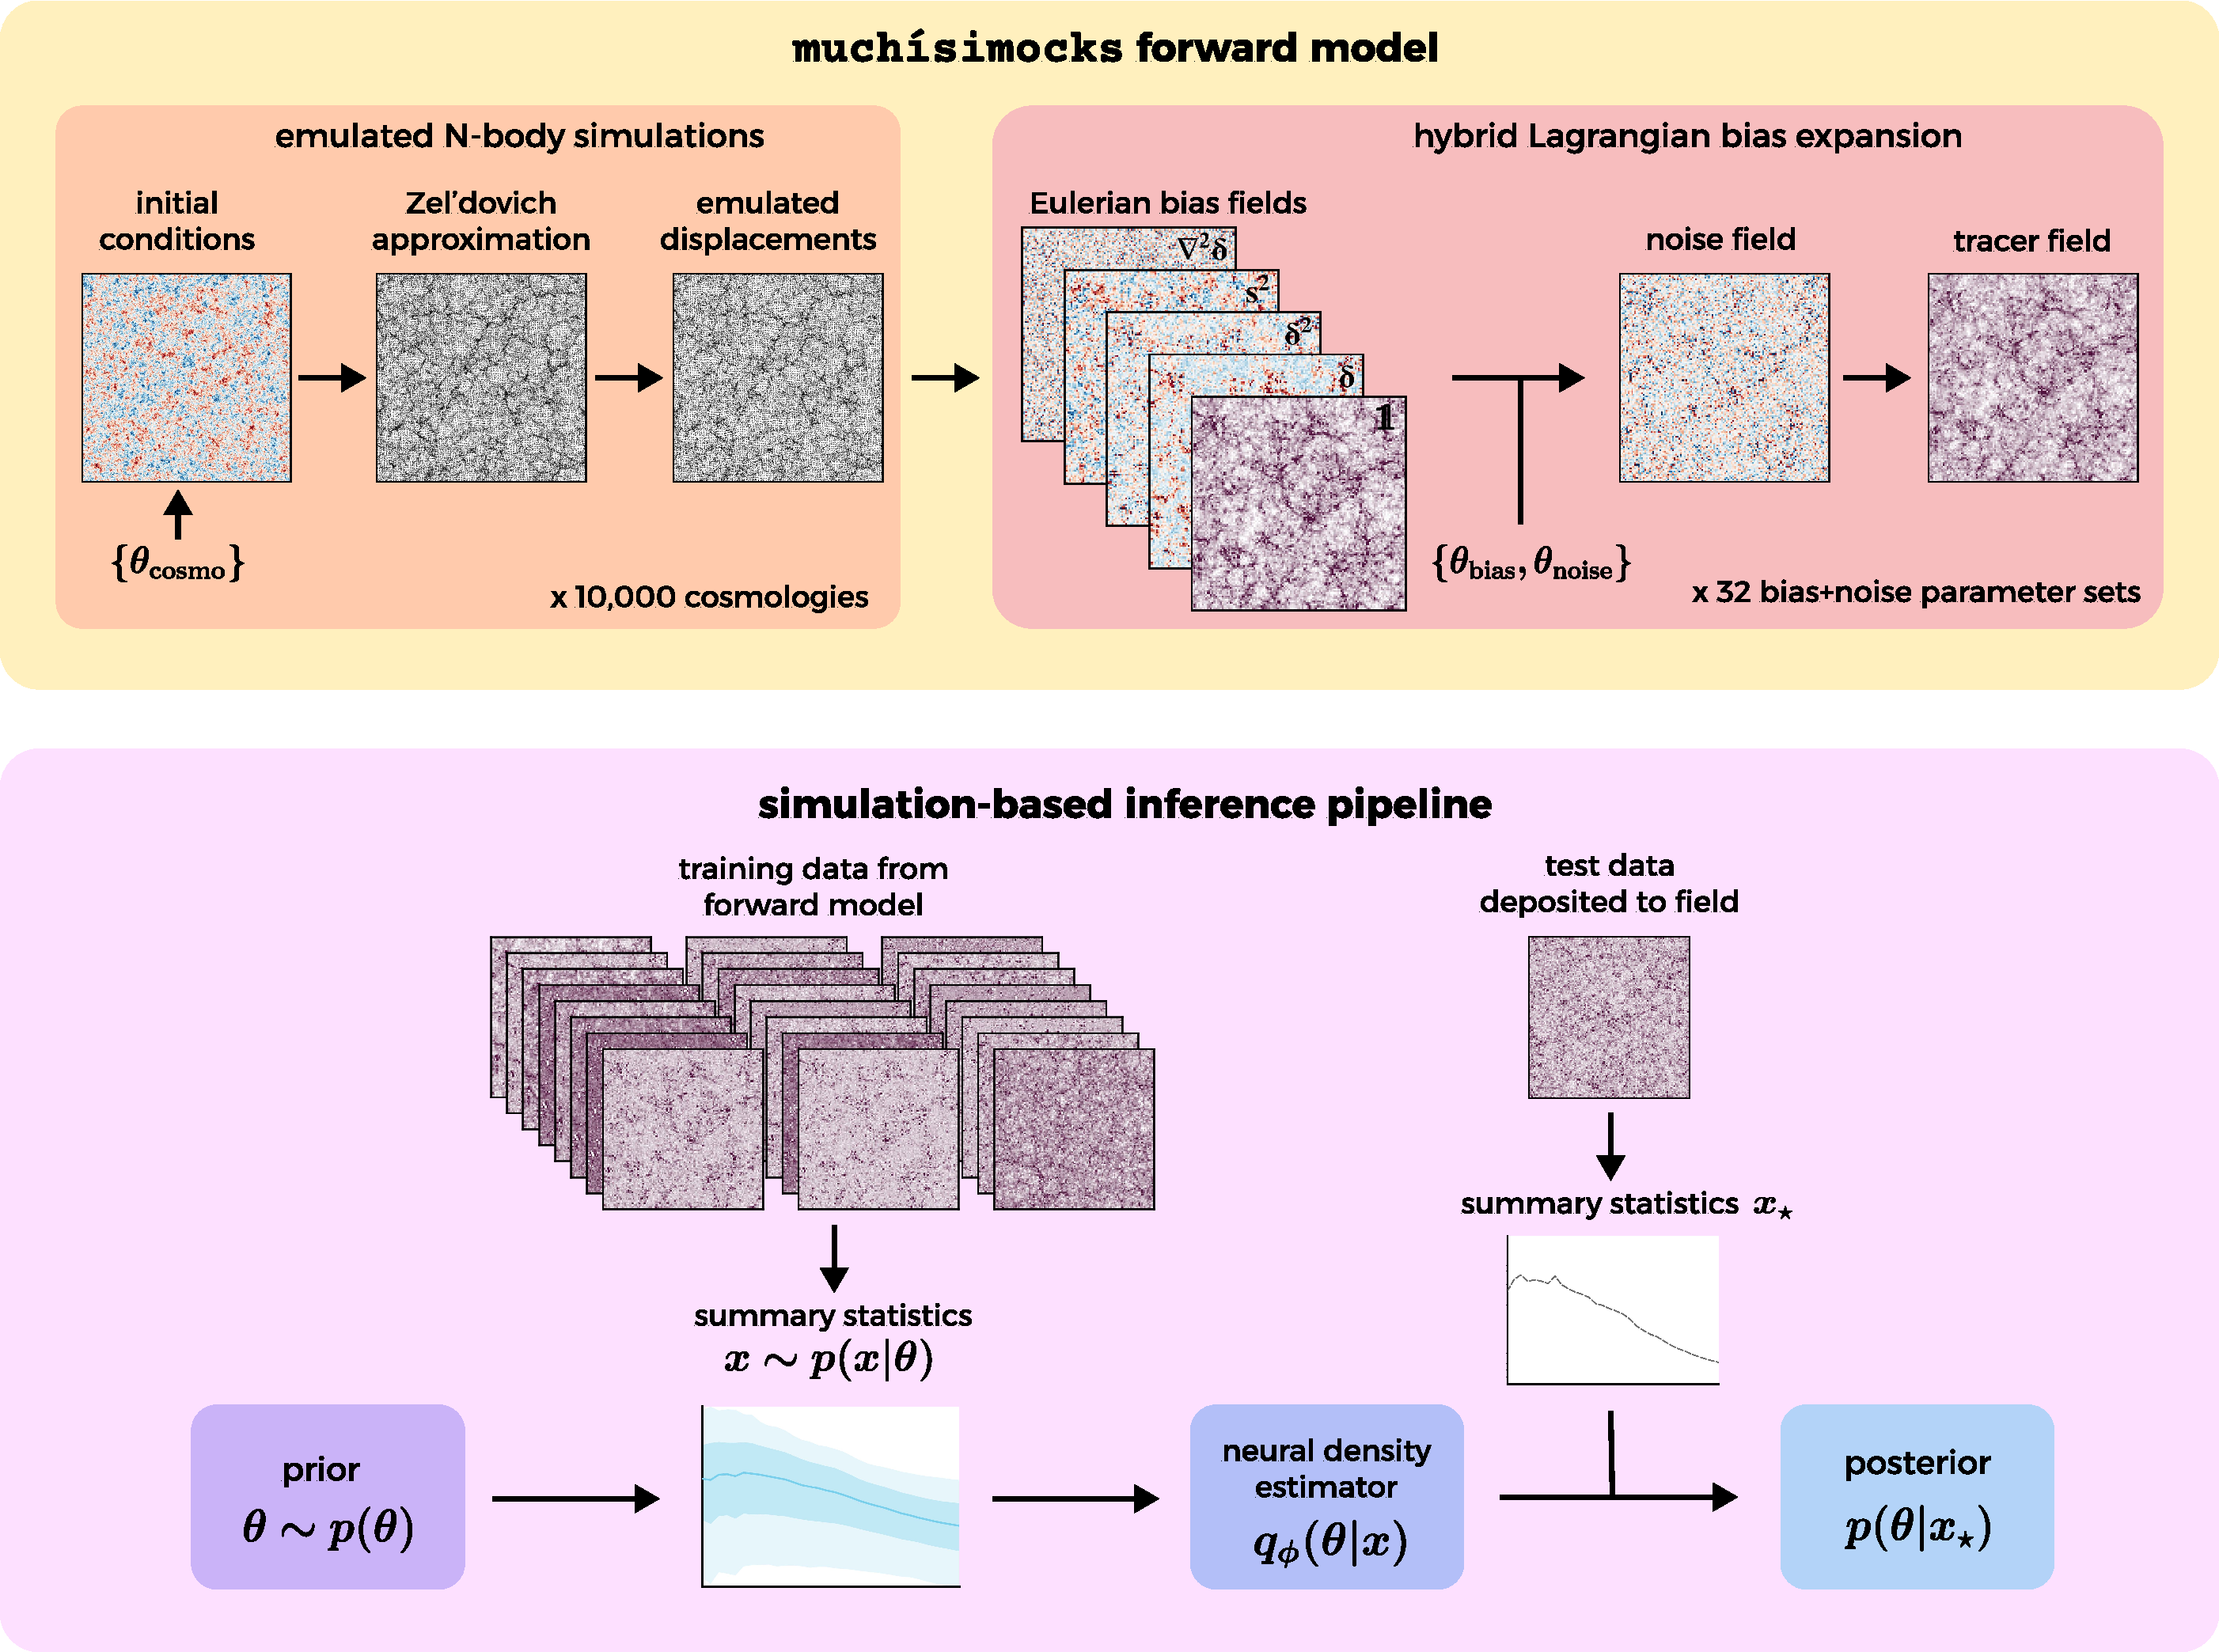
\includegraphics[width=\textwidth]{figures/fig1_schematic.pdf}
\caption{Schematic overview of the \mmocks suite and simulation-based inference pipeline. For our forward model, we start with an initial conditions field based on input cosmological parameters, and apply the Zel'dovich approximation; these are passed to \mtm which emulates the $N$-body displacement field. Using these as inputs to the hybrid Lagrangian bias expansion, we produce second-order Lagrangian bias fields advected to Eulerian space; these compose the core of the \mmocks suite. These are then combined with a choice of bias parameters, as well as a full-field noise model. The combined tracer fields and associated parameters are used to train a neural posterior estimator, which conditioned on test data can then predict the associated parameters.}
\label{fig:schematic}
\end{figure*}

\subsection{Emulating the displacement field with \mtm}
\label{sec:mtm}

The nonlinear matter distribution can be simulated to high accuracy with $N$-body simulations.
However, simulations with the resolution and volume required to analyze current galaxy surveys are very expensive, and training simulation-based inference models requires a very large  of simulations.
We thus turn to a field-level emulator of the matter distribution, \mtm \citep{jamieson_field_2023}.

The density field can be approximated at linear order by the Zel'dovich approximation (ZA, also known as first-order Lagrangian perturbation theory, 1LPT), based on a realization of an initial conditions field.
The \mtm emulator learns a mapping from the ZA field at $z=0$ to the non-linear $N$-body displacement field at that redshift, effectively learning the correction from linear to non-linear displacements. 
The emulator is trained on 2000 simulations of the Quijote simulation suite that span a Latin hypercube (LH) of five cosmological parameters: $\Omega_\mathrm{c}$, $\sig$, $\h$, $\ob$, and $n_\mathrm{s}$  \citep{villaescusa-navarro_quijote_2020}.
Each has a volume of (1 $\hinv$Gpc)$^3$ with $512^3$ particles, giving particle mass resolutions in the range $2 \times 10^{11} - 1 \times 10^{12} \hinv M_\odot$.
\mtm also trains a separate network to predict the nonlinear velocity field from the ZA velocities.
For this work, we use a modified version of this velocity prediction: following the $\bacco$ model, we assign Lagrangian particles that end up in halos as all having the same velocity, that of the center-of-mass velocity of the parent halo (see \cite{pellejero_ibanez_hybrid-bias_2023} for details). \ksf{please check this sentence!}
Once trained, \mtm can generate the displacement and velocity fields for any input ZA field, taking a few minutes on a GPU for a (1 $\hinv$Gpc)$^3$ volume.
While we do not utilize the velocity fields in this work, as we limit to real-space analysis, these will be important for future analyses including redshift-space distortions as well as other applications involving the velocity distribution; we release them as part of the \mmocks suite.

In more detail, \mtm consists of two convolutional neural networks (CNNs), one to predict the matter density field and the other to predict the velocity field.
The particle displacements are structured on a 3D grid as they are functions of their initial Lagrangian space position, so the CNN processes the inputs and outputs as 3-channel images.
As most of the cosmological parameters only affect the input power spectrum that is used to create the ZA field, these are not needed as additional inputs to the model.
However, the matter density $\om$ affects the N-body evolution, so is included as an input ``style'' parameter; this is incorporated via the approach of the StyleGAN2 \citep{karras_analyzing_2020}, in which the style parameters modulate the convolution kernels.
The model uses a V-net-like architecture, with 3 layers of downsampling and upsampling, and leaky ReLU activations.
For its loss function, it combines the log mean squared error of the Lagrangian particle displacements and Eulerian density field.
We note that there is a newer version of \mtm that includes redshift dependence, and predicts the velocity field as a derivative of the position field \citep{jamieson_field-level_2024}; however, as we focus on $z=0$ and also require a modification of the velocity field as described above, we use the original \mtm implementation.

For our mock suite, we define a Latin hypercube of 10,000 sets of cosmological parameters: $\Omega_\mathrm{c}$, $\sig$, $\h$, $\ob$, and $n_\mathrm{s}$.
We use uniform priors for each parameter that span $\sim$10 around the \cite{collaboration_planck_2014} values of the cosmological parameters, following \cite{Angulo2021} (with a range for $\sig$ extended to slightly lower values); these are shown in Table~\ref{tab:priors}.
For each of these, we generate a ZA field based on a different random seed, and pass that field through map2map to obtain the nonlinear particle displacements.
The \mtm-emulated particle displacements are a key ingredient in modeling the galaxy bias fields, as discussed in the next section.


\subsection{Modeling tracers with the hybrid bias expansion}
\label{sec:hbe}

To model biased tracers of the matter field, we use the hybrid Lagrangian bias expansion, also known as hybrid effective field theory (HEFT, \citealt{modi_simulations_2020, kokron_cosmology_2021, zennaro_bacco_2023}).
We first define a mapping from initial (Lagrangian) space coordinates $\qq$ to Eulerian space coordinates $\bm{x}$ as $\bm{x} = \qq + \Psi(\qq)$, where $\Psi(\qq)$ is the Lagrangian space displacement field.
This advection from Lagrangian to Eulerian space effectively expresses the overdensity field as weighted contributions fom the initial density field that end up in a given Eulerian location.
The displacement term $\Psi(\qq)$ can be computed with Lagrangian perturbation theory, but this is only accurate down to mildly non-linear scales; here we take the ``hybrid'' approach which uses $N$-body displacements to compute $\Psi(\qq)$, significantly improving the accuracy down to non-linear scales.

The galaxy overdensity field in Lagrangian space can be described to second order as 
\begin{equation}
\begin{split}
\delta_g(\qq) = 1 + \bo \delta_L(\qq) + \bt \left[ \delta_L^2 (\qq) - \langle \delta_L^2 \rangle \right] \\
+ \bs \left[s^2(\qq) - \langle s^2 \rangle \right] + \bl \nabla^2 \delta_L(\qq)
\end{split}
\label{eq:hbe}
\end{equation}
where $\delta_L(\qq)$ is the linear matter density in Lagrangian space, and $s^2(\qq)$ is the shear field, defined by the traceless part of the tidal field, given by $s^2(\qq) = s_{ij}(\qq) s^{ij}(\qq) = \delta_i \delta_j \phi(\qq) - \frac{1}{3}\delta^K_{ij} \delta_L(\qq)$, where $\phi(\qq)$ is the linear gravitational potential in Lagrangian space $\nabla^2 \phi(\qq)=4 \pi G \bar{\rho} \delta_L(\qq)$, and $\delta^K$ is the Kronecker delta.
The coefficients $\bo$, $\bt$, $\bs$, and $\bl$ are the Lagrangian bias parameters.
The prior ranges of the bias parameters used in our SBI analysis are shown in Table~\ref{tab:priors}, though we note that a tracer field could be constructed for any choice of bias parameters with our saved bias fields.

We build this field starting from a random realization of the initial Gaussian field on a $N_\mathrm{grid} = 512^3$ grid in a $L = (1 \Gpch)^3$ box, matching the resolution and size of the Quijote simulations that \mtm was trained on, and use the ZA to compute approximate displacements.
We pass the ZA displacement and velocity fields as input to \mtm (\S\ref{sec:mtm}), which outputs emulated $N$-body displacement and velocity fields.
We compute the Lagrangian operators based on the linear density field, smoothing these with a damping scale of $k=0.75 \hMpc$.
We then perform the advection to Eulerian space: The tracers are deposited onto a grid in Eulerian space with a cloud-in-cell (CIC) assignment, with positions given by the simulation displacement field and weights given by Lagrangian operator.
This gives five bias fields in Eulerian space, $\mathcal{O}_i$: weighting the Lagrangian density field by the constant 1 gives the homogeneous field; by $\delta_L(\qq)$, the linear density field; by $\delta_L^2 (\qq) - \langle \delta^2 \rangle$, the quadratic density field; by $s^2(\qq) - \langle s^2 \rangle$, the tidal field; and by $\Delta^2 \delta(\qq)$, the Laplacian.
These fields can be weighted by the bias coefficients and summed to produce an overall tracer field $\delta_g$.

We perform two postprocessing steps on these fields.
To reduce storage space, we reduce the size of these fields by cutting the high-$k$ modes: we remove modes beyond $k_\mathrm{Nyquist} = \pi N_\mathrm{grid,cut} / L \approx 0.4$, where $N_\mathrm{grid,cut}=128$, our reduced grid size.
We do this by Fourier transforming each bias field, nulling the modes higher than $k_\mathrm{Nyquist}$, and inverse Fourier transforming back to real space.
At scales higher than this our hybrid bias model loses accuracy anyway and we don't consider them in our inference, so we do not give up accuracy with this $k$-cut.
We perform the same reduction on the velocity fields, cutting each component of the velocity vectors in $k$-space.
We finally perform a deconvolution of the bias fields, using a linear interpolation kernel at the original grid size $N_\mathrm{grid}$ to correct for the smoothing by the CIC kernel.
(Technically the deconvolution should be performed before the $k$-cut, but we confirm the results are effectively equivalent and this ordering is much faster.)
This deconvolution could be done at the summary statistics level, but we choose to deconvolve the fields for ease of use.

The final main suite, designed as a training set, contains 10,000 sets of tracer position fields (5 Lagrangian bias fields advected to Eulerian space) and velocity fields, each at a different cosmology; each is of size $(1 \Gpch)^3$ and resolution $128^3$.
We also generate multiple smaller suites for testing, detailed in \S\ref{sec:testsets}.
We call these suites \mmocks (a portmanteau of the words ``much\'isimos'', Spanish for ``many'', and ``mocks'').


\subsection{Modeling noise at the field level}
\label{sec:noise}

\ksf{technically this is a postprocessing step only needed for the SBI part, is it fine here?}

We require a model for stochastic noise in order to model realistic discrete galaxy populations.
This can be modeled at the level of each summary statistic, but our goal is to make this suite usable for a wide range of statistics as well as field-level analyses; we thus desire a field-level noise model.
Further, as we are considering higher-order statistics, we need to include non-Gaussian noise contributions.
We thus turn to the noise model of \cite{rubira_non-gaussian_2025}, an EFT approach described by nonlinear couplings of a single Gaussian field to the bias fields. 
In this model the galaxy density field can be written as
\begin{equation}
    \delta_g(\mathbf{x}) = \sum_{m=0}^{\infty} \sum_{1,\mathcal{O}} b_\mathcal{O}^{\{m\}} \left[ \epsilon_G(\mathbf{x}) \right]^m \mathcal{O}(\mathbf{x})
\label{eq:noise}
\end{equation}
where $m$ is the order of the expansion in the noise field, $\epsilon_G(\mathbf{x}) = \mathcal{N}(O,1)$ is a unit Gaussian field, $\mathcal{O}$ are operators of the galaxy density field, and $\{b_\mathbb{1}^{\{m\}}, b_\mathcal{O}^{\{m\}}\}$ are free coefficients.
In our case we limit to second order in the bias expansion, as described in \S\ref{sec:hbe}; limiting to zeroth order in $m$ reduces to the noiseless case, as in Equation~\ref{eq:hbe}.
For our SBI analysis, we include terms through first order in the noise expansion, $m=0,1$.
That gives us bias coefficients \{$b_\mathcal{O}^{\{0\}}\} =$ $\bo$, $\bt$, $\bs$, $\bl$, as in Equation~\ref{eq:hbe} (we fix $b_\mathbb{1}^{\{0\}}=1$), and noise coefficients \{$b_\mathcal{O}^{\{1\}}\} =$ $\Ah$, $\Ao$, $\At$, $\As$, $\Al$. 

We note that limiting the noise model to $m=1$ means that we exclude noise contributions to $\pgm$, as at $m=1$ the noise field $\epsilon_G$ has zero mean (whereas $\pk$ and $\bispec$ get factors of $\epsilon_G^2$ which don't vanish).
This means that the bias parameters may have to absorb partial noise contributions, though we show that we still achieve largely unbiased bias parameters; future work could extend this noise model to $m=2$ or choose a well-motivated subset of noise parameters tailed to the statistics analyzed.

Operationally, we generate one unit Gaussian noise field $\epsilon_G$ per cosmology in our suite.
We store these and use them to construct the noisy tracer field on-the-fly just before computing the summary statistics of the field.
This means that we use the same noise realization when we select different bias and noise parameter sets for the same cosmology (detailed in \S\ref{sec:trainingsets} and \S\ref{sec:testsets}), which introduces some undesirable non-independence; however, we expect the effects of this to be minimal, and the storage cost of one noise field per bias model is prohibitive.
The prior ranges of the noise parameters used in our SBI analysis are shown in Table~\ref{tab:priors}.


\section{Simulation-based inference methodology}
\label{sec:sbi}

\subsection{Neural posterior estimation}
\label{sec:npe}

The main idea behind simulation-based inference is that we can infer a posterior distribution of our data over the parameters of interest using only a \emph{simulator}, which produces data samples given a set of parameters.
This is distinct from explicit likelihood inference, in which we are required to define a likelihood of our data with respect to the parameters.
Neural density estimators (NDEs) present a flexible and robust way to model a target distribution.
Here, we use neural posterior estimation, which uses an NDE to directly model the posterior distribution.

To do this, we aim to minimize the distance between the true posterior $\post$ and the NDE model of the posterior $\qpost$, where $\phi$ are the parameters of the neural network model.
We use maximum likelihood estimation, which minimizes the Kullback-Leibler divergence between the distributions.
In practice, we consider the posteriors multiplied by $p(x)$, and use the fact that $\post p(x) = p(\theta,x)$:

\begin{equation}
\begin{aligned}
\min_{\phi} D_\mathrm{KL}\bigl(\post \,\Vert\, \qpost\,p(x)\bigr)
&= \min_{\phi} \int p(\theta,x)\,\log\frac{\post}{\qpost}\,d\theta\,dx \\
&\approx \min_{\phi} \sum_i \log p(\theta_i|x_i) - \log q_\phi(\theta_i|x_i) \\
&\approx \min_{\phi} \sum_i -\log q_\phi(\theta_i|x_i) \\
&\approx \max_{\phi} \sum_i \log q_\phi(\theta_i|x_i)
\end{aligned}
\label{eq:loss}
\end{equation}

where in the second line, we perform a Monte Carlo expectation of the integral using discrete samples from our simulation (dropping the $\frac{1}{N}$ as it does not affect the minimization); in the third line, we observe that we are minimizing with respect to the neural network parameters $\phi$ and the true posterior $\post$ is independent of $\phi$ so it drops out; and in the final line we use the fact that minimizing the positive is the same as maximizing the negative.

Normalizing flows are a popular choice for the NDE, thanks to their expressivity and flexibility.
The key idea is to transform an initial simple distribution into the target distribution through a chain of transformations.
A normalizing flow is defined as
\begin{equation}
    q_\phi(\theta \mid x) = \pi_z\big(f^{-1}(\theta, x)\big) \left| \det \left( \frac{\partial f^{-1}}{\partial \theta} \right) \right| ~,
\end{equation}
where $f$ is an invertible transformation modeled as a neural network and $\pi_z$ is a base distribution, for which we follow the common choice of a Gaussian, $\pi_z(z) = \mathcal{N}(z|\mathbf{0}, \mathbf{I})$.
The Jacobian (the determinant term) arises from the change of variables, and involves $f^{-1}$, thus requiring $f$ to be invertible.
The invertibility property of NFs both enables us to sample from the network and gives us an explicit density, which is key for performing SBI.

Specifically, we use masked autoregressive flows (MAFs), which stack Masked Autoencoders for Distribution Estimation (MADEs) in order to model more complex distributions:
\begin{equation}
    q_\phi(\theta \mid x) = \pi_z(z_0) \prod_{t=1}^T \left| \det \left( \frac{\partial f_t^{-1}}{\partial z_t} \right) \right|~,
\end{equation}
where $z_0 \sim \pi_z$, $t$ indexes the MADE blocks, and each network $f_t$ takes as input the previous variable $z_{t-1}$ as well as the observation $x$, the final layer is identified with the parameters, $z_T \equiv \theta$.
The loss function derived from the KL divergence (Equation \ref{eq:loss}) is used to train the network and learn the optimal weights and biases.


\subsection{Training set}
\label{sec:trainingsets}

To train our simulation-based inference model, we use the main \mmocks suite of bias fields to generate a set of tracer fields.
Our prior on the cosmological parameters is set by the range of the suite, as described in \ref{sec:mtm}. 
We need to define the range of the bias coefficients $\{b\}$ we use to sum the fields; for this, we use the results of \cite{zennaro_priors_2022}, which define priors that capture a range of realistic galaxy populations modeled with the extended subhalo abundance matching technique \cite{contreras_flexible_2021}.
We choose to use uniform priors with slightly wider ranges than the relations found by \cite{zennaro_priors_2022}, a more conservative choice; these prior ranges are shown in Table~\ref{tab:priors}.
For the noise coefficients $\{A^\mathrm{noise}\}$ we choose wide uniform priors loosely based off of the corresponding (noiseless) bias coefficients.

\begin{table}
\centering
\caption{Uniform prior ranges for the cosmological, bias, and noise parameters. The cosmological parameters are based on a $\sim$10 range around the \citet{collaboration_planck_2014} best-fit values, and the bias and noise parameters are loosely based on the hypervolume found by \citet{zennaro_priors_2022} for a wide range of realistic galaxy populations.}
\label{tab:priors}
\begin{tabular}{lcc}
\toprule
Parameter & Lower bound & Upper bound \\
\midrule
\multicolumn{3}{l}{\textit{Cosmological parameters}} \\
\midrule
$\Omega_\mathrm{c}$ & 0.23 & 0.40 \\
$\sig$ & 0.65 & 0.90 \\
$\h$ & 0.6 & 0.8 \\
$\ob$ & 0.04 & 0.06 \\
$n_\mathrm{s}$ & 0.92 & 1.01 \\
\midrule
\multicolumn{3}{l}{\textit{Bias parameters}} \\
\midrule
$\bo$ & $-$1.0 & 3.0 \\
$\bt$ & $-$2.0 & 2.0 \\
$\bs$ & $-$2.0 & 2.0 \\
$\bl$ & $-$10.0 & 10.0 \\
\midrule
\multicolumn{3}{l}{\textit{Noise parameters}} \\
\midrule
$\Ah$ & $-$3.0 & 3.0 \\
$\Ao$ & $-$3.0 & 3.0 \\
$\At$ & $-$2.0 & 2.0 \\
$\As$ & $-$5.0 & 5.0 \\
$\Al$ & $-$10.0 & 10.0 \\
\bottomrule
\end{tabular}
\end{table}

While we are limited to the 10,000 cosmologies defined in the \mmocks suite, we can combine these into tracer fields with any number of bias parameter sets we choose.
At a given cosmology, we then have multiple tracer fields generated with distinct sets of bias and noise parameters.
Though this means the final tracer fields are not fully independent of each other, this has been shown (e.g. in \cite{hahn_rm_2023-2}) to improve inference by significantly augmenting the training data size and allowing the model to disentangle cosmology and bias parameters.
Note that the summing of bias fields with the chosen bias coefficients is essentially instantaneous and can be done in postprocessing just before computing summary statistics, and thus requires no additional compute time or storage.

As we later want to test convergence of the inference with the number of bias parameter sets, we use a \emph{nested Latin hypercube} to generate the bias parameters.
The top-level LH contains 320,000 points, resulting in 32 independent bias parameter sets for each of the 10,000 cosmologies.
Nested subsets of this LH are also LHs, with 16, 8, 4, 2, and 1 bias parameter sets per cosmology.
We generate one nested LH for the noiseless case with the 4-parameter set of bias parameters; and a separate nested LH for the noisy case with 4 bias parameters and 5 noise parameters, for a total of 9 independently varied parameters.

This was achieved with the \cite{qian_nested_2009} algorithm for nested Latin hypercubes, which works by starting with a two-layer structure, with coarse cells and fine cells on a multidimensional grid. 
It constructs a standard LH on the coarse cells, and then fills in the finer grid, also ensuring it creates a valid LH.
It then performs random permutations of rows and cells that still preserve the LH structure but remove any deterministic structure from the filling procedure, resulting in a random realization of two nested LHs. 
This is then repeated for subsequent layers by adding finer and finer grids.
A python implementation of this algorithm along with validation tests are available in the \texttt{gethypercube}\footnote{http://github.com/kstoreyf/gethypercube} package.
\ksf{i may include an appendix detailing my nested-LH package! thoughts?}
Though the LHs at all levels are exact, they are not guaranteed to have optimal space-filling properties compared to an optimized single-level LH; however, this nested design is shown to achieve LHs at each level that have properties much closer to a true LH than either taking random subsets of a top-level LH, or stacking bottom-level LHs.
The use of LH-distributed parameters has been shown to be important for accurate and robust training, so we expect that this nested strategy leads to robustness in our convergence tests, which are a key result of this work.

To generate our final tracer fields, we weight the \mmocks bias fields and noise field by the selected set of corresponding bias and noise parameters as in Equation~(\ref{eq:noise}), and sum these weighted fields.
We normalize these fields by the original \mtm grid size ($512^3$) before computing their summary statistics.


\subsection{Summary statistics}
\label{sec:stats}

We perform our SBI analysis with our \mmocks framework on three standard summary statistics: the galaxy--galaxy power spectrum $\pk$, the galaxy--matter power spectrum $\pgm$, and the bispectrum $\bispec$.

The galaxy--galaxy auto power spectrum $\pk$ is defined by
\begin{equation}
    \langle \delta_g(\bm{k}) \delta_g(\bm{k}') \rangle = (2\pi)^3 \delta_{\mathrm{D}}(\bm{k}+\bm{k}') P_{gg}(k) ~,
\end{equation}
where $k = |\bm{k}|$ is the Fourier space wavenumber.
This is the two-point function of the galaxy field, the most common statistic for cosmological inference from galaxy samples that captures all the Gaussian information.
We use 32 logarithmically spaced bins from $k=0.01$ to $k=0.4$; the maximum $k$ value is set by the Nyquist frequency of our mocks. 
We use the \bacco code to compute $\pk$ for our mocks.
We can compute the 15 cross-terms of the 5 bias fields and later sum their contributions based on the bias parameters to obtain the power spectrum of the total tracer field; in practice we do this for the noiseless case, but in the noisy case compute $P_{gg}(k)$ for the total tracer field as this would add additional terms.

The galaxy--matter cross power spectrum $\pgm$ is defined by
\begin{equation}
    \langle \delta_g(\bm{k}) \delta_m(\bm{k}') \rangle = (2\pi)^3 \delta_{\mathrm{D}}(\bm{k}+\bm{k}') P_{gm}(k) ~,
\end{equation}
where $\delta_m(\bm{k})$ is the matter density field in Fourier space.
This represents the galaxy-galaxy lensing contribution to 3x2pt analyses, and is critical for constraining galaxy bias and breaking parameter degeneracies.
We use the same binning as $\pk$, and again use the \bacco code to compute $\pgm$ for our mocks; for our fiducial results, we only use up to $\kmax=0.25$ for $P_{gm}(k)$.

The galaxy auto-bispectrum $\bispec$ is defined by
\begin{equation}
    \langle \delta_g(\bm{k}_1) \delta_g(\bm{k}_2) \delta_g(\bm{k}_3) \rangle = (2\pi)^3 \delta_{\mathrm{D}}(\bm{k}_1+\bm{k}_2+\bm{k}_3) B_{ggg}(k_1,k_2,k_3) ~.
\end{equation}
This is the Fourier space three-point function.
We choose 12 linearly spaced bin edges from $k=0.01$ to $k=0.4$, yielding 203 triangles; for our fiducial results, we only use triangles with edges up to $\kmax=0.25$, yielding 50 triangles.
We use the \texttt{PolyBin3D} code \citep{philcox_polybin3d_2024} to compute $\bispec$ for our mocks.

The summary statistics computed on the \mmocks training set are shown in Fig.~\ref{fig:statistics_ranges}.

\begin{figure*}
\centering
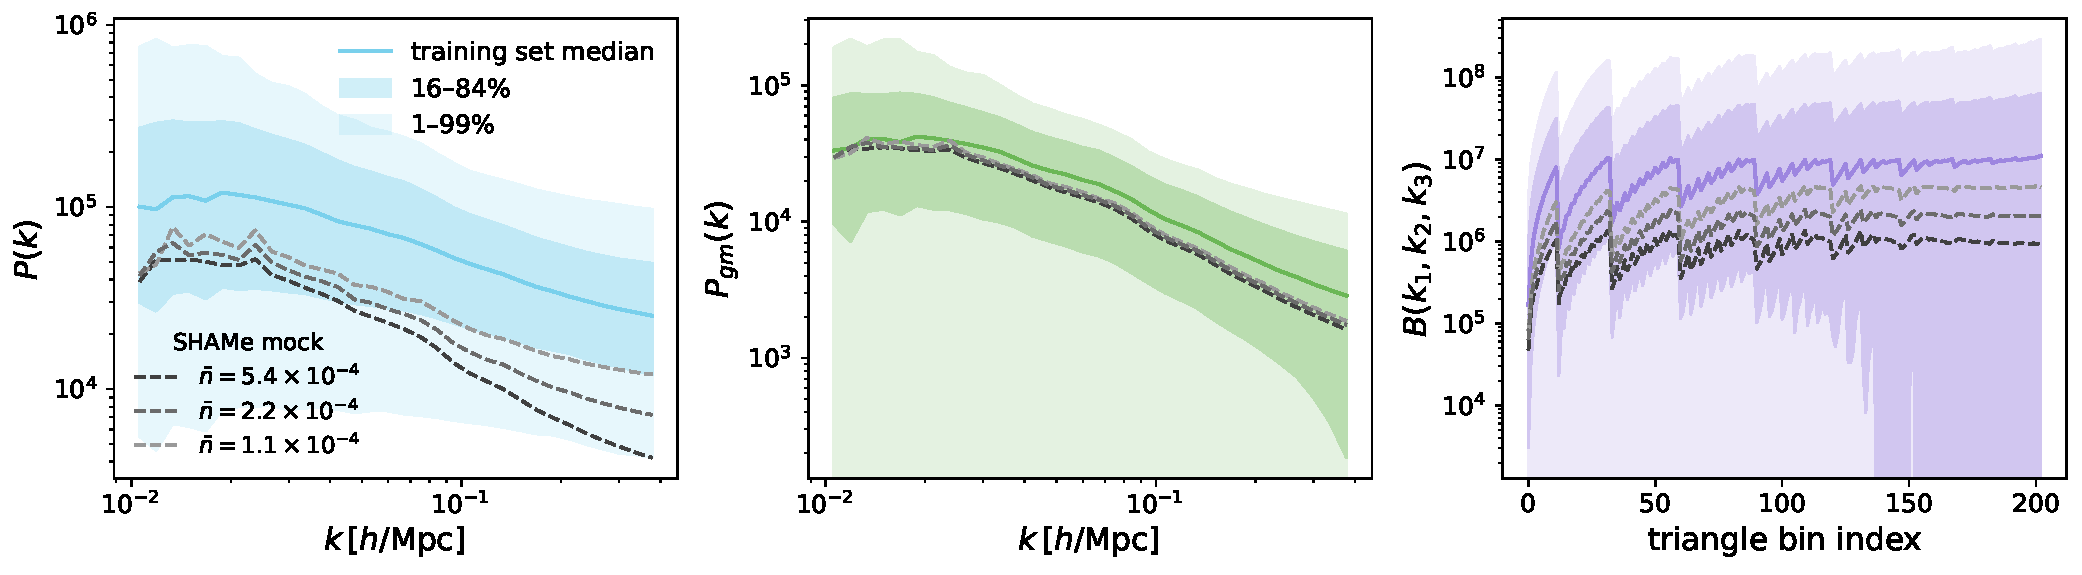
\includegraphics[width=\textwidth]{figures/fig2_statistics_ranges.pdf}
\caption{The summary statistics computed on the \mmocks training set: the galaxy--galaxy power spectrum $\pk$, the galaxy--mater power spectrum $\pgm$, and the galaxy bispectrum $\bispec$. The median, 16th-84th percentiles, and 5th-95th percentiles of the training set. The out-of-distribution test mock catalog constructed with extended subhalo abundance matching (SHAMe) on a \bacco simulation is also shown (black dashed). In our fiducial inference model, scales below $\kmax=0.25$ for $\pgm$ and triangles with sides smaller than $\kmax=0.25$ for $\bispec$ are excluded.}
% \ksf{double check shame; maybe if have b2 thats very large? pgm: avg b1*p11 matches shame. for pk, avg b1**2 * p11 doesnt match. or, addl operators that appear in pgg and not pgm; aka p22. usually its smaller, but for v broad prior (aka b2 goes up to 2), then part of param space where p22. so could be because of prior. test: do same plot but restrict b2 from -1 to 0.}
\label{fig:statistics_ranges}
\end{figure*}

\subsection{Implementation and training}

Before training, we reparameterize the cosmology and bias parameters to combinations that are better constrained by the summary statistics, and thus should result in improved training convergence.
We multiply the bias and noise parameters by the relevant power of $\sig$, obtaining $\sig \bo$, $\sig^2 \bt$, $\sig^2 \bs$, $\sig \bl$, $\sig \Ao$, $\sig^2 \At$, $\sig^2 \As$, and $\sig \Al$.
When sampling from the posterior, we can divide out the appropriate power of the recovered $sig$ to obtain estimates of the original bias and noise parameters.
We also do not include the cosmological parameters $\h$, $\ob$, and $n_\mathrm{s}$ in the SBI training, as we do not expect to constrain these parameters (and confirmed in tests); these are still varied in the training set and implicitly marginalized over.

We use the publicly available \texttt{sbi} \cite{tejero-cantero_sbi_2020} package for the NPE and MAF implementations \citep{papamakarios_fast_2016, greenberg_automatic_2019}; the MAF uses the nflows Python package \citep{durkan_neural_2019, durkan_contrastive_2020}.
Our data vector is comprised of the binned statistics discussed in \S\ref{sec:stats}, concanenated when using multiple statics. 
The statistics combinations we show are: $\pk$, $\pk+\bispec$, $\pk+\pgm$, $\pk+\bispec+\pgm$ (we exclude $\bispec$ and $\pgm$ alone, as these do not contain much constraining power on their own and in practice are almost always considered in combination with $\pk$). 
We use a 90\%/10\% training/validation split of our training set.
We use the \textsc{Adam} optimizer, and stop training when the mean loss over the validation set does not improve for 20 epochs; we save the network weights at the best validation loss.

We perform a sweep over several hyperparameters, using 30 random samples from the following sets: the learning rate $\{10^{-2},\,3\times10^{-3},\,10^{-3},\,3\times10^{-4},\,10^{-4},\,3\times10^{-5},\,10^{-5}\}$, hidden features $\{32,\,64,\,128,\,256\}$, training batch size $\{32,\,64,\,128,\,256\}$, and number of transforms $\{4,\,6,\,8,\,10\}$. 
The sweeps are performed separately for each statistic or combination of statistics, and for each choice of noiseless (bias parameters only) and noisy (bias and noise parameters) training data; we use the maximum size training set of 320,000 data vectors, and for the statistics use $k_{\mathrm{max}}^{P_{gg}}=0.37$, $k_{\mathrm{max}}^{P_{gm}}=0.25$, and $k_{\mathrm{max}}^{B}=0.25$.
We look at the ordered mean validation losses of the 30 trained models for each statistics combination, and observe a signficant drop for the top three models (this number will vary depending on the number models explored in the sweep and is generally chosen empirically).
We thus choose to use an equally weighted ensemble of the top three MAFs when performing inference, which has been shown to lead to more stable results (e.g. \citealt{alvey_simulation-based_2026}); explicitly, we sample the MAFs as $q_\phi(\theta \mid x) = \frac{1}{3}\sum_{j=1}^{3} q_\phi^{j}(\theta \mid x)$.
We use the sets of hyperparameters from the three top MAFs to train variations of the model for the given statistics combination, such as when varying the number of training points and the $\kmax$ values, rather than running dedicated sweeps which would be computationally very expensive.
The set of best identified hyperparameters vary across the statistics, with the noisy case (which varies more parameters) generally preferring larger hidden feature vectors and batch sizes, though most learning rates are around $10^{-4}$.

Training one MAF on the maximum size training set of 320,000 data vectors takes a few hours on a single CPU for the fiducial model described abve.
To display the posteriors and compute covariances and other statistics from them, we draw 10,000 samples from the posterior; we confirm that the posteriors are generally converged with this number of samples.


\subsection{Test sets}
\label{sec:testsets}

We generate several test sets to validate our \mmocks suite and our SBI approach.

Our first test set is a \emph{cosmic variance set}.
For this we use \mmocks pipeline to construct 1000 additional mocks each with a different random seeds, all at the same fixed cosmology; we choose this to be the same cosmology as the out-of-distribution SHAMe mock test described below.
We fix the bias parameters to those measured from that mock, and use these to combine the bias fields into a tracer field for each realization.
For the noise parameters, we cannot measure these from the mock directly; to identify realistic noise parameters, we generate 1000 sets of noise parameters and add the resulting noise field to each of the 1000 mocks, obtaining tracer fields that have the same cosmology and bias parameters but different noise parameters. 
We compute the statistics of these fields, and then compute the reduced $\chi^2$ between them and the statistics of the SHAMe mock. 
Specifically, we use $\pk$ and $\bispec$ with the fiducial $\kmax$ choices (the noise model does not affect $\pgm$ as discussed in \S\ref{sec:noise} so we exclude it), and  choose the set of noise parameters that gives the lowest $\chi^2$. 
We then use this set of noise parameters and regenerate the noise fields with different noise realizations, and combine this with the biased tracer fields to obtain our final set of 1000 cosmic variance mocks at fixed cosmology, bias, and noise parameters, only varying the random seeds.
For the recovery tests, we compute the mean statistic over these 1000 mocks, and perform SBI on that mean to reduce the randomness from cosmic variance; in Appendix~\ref{sec:meandemo} we show that this gives the same result as combining the results of inference on each of the 1000 mocks, while being much faster.

Our second test set is our \emph{coverage set}.
This consists of 1000 mocks generated with the \mmocks pipeline that span the same prior range of cosmology, bias, and noise parameters as in the training set.
To select the parameters, we construct an independent 1000-point LH for the cosmologies, and a separate LH for the bias and noise parameters.
The coverage set tests the performance of our method across the prior space and its dependence on the parameter values.

Our final test set is our \emph{SHAMe mock}; we construct a realistic catalog of galaxies using the extended subhalo abundance matching (SHAMe) approach \cite{contreras_flexible_2021} applied to a \bacco $N$-body simulation \cite{Angulo2021}.
This is a stringent test as it uses both a different, signficantly higher resolution underlying cosmological simulation and a completely different galaxy formation model than the \mmocks data used to train the inference network, testing the generalizability of our model.
In detail, we use a simulation with a box size of (1024 $\hinv$Mpc)$^3$ (slightly larger than the \mmocks training data) and $3072^3$ particles, which uses the fixed-and-paired technique \citep{Angulo2021}, and has Planck cosmology $\Omega_\mathrm{c}=0.309$, $\sig=0.816$, $\h=0.677$, $\ob=0.0486$, and $n_\mathrm{s}=0.967$ \citep{collaboration_planck_2014}.
Halos are identified using a variant of the \textsc{SUBFIND} halo finder \citep{springel_populating_2001}, and we populate these halos with galaxies using the SHAMe model with the following parameter choices: $\sigma_\mathrm{logM}=0.47513517$, $t_\mathrm{merger}=-0.4577029$, $f_\mathrm{k,cen+sat}=0.20147321$, $f_\mathrm{k,cen-sat}=-0.02964998$, $\beta_\mathrm{lum}=14.82600407$.
We choose a fiducial number density of $\nbarfid$, similar to that of DESI luminous red galaxies (LRGs) when scaled to $z=0$. \ksf{checking that this is right? also are the shame parameters chosen to be lrg-like?}
To check our inference results, we measure the bias parameters of this sample using the field-level probabilistic bias approach of \cite{stucker_probabilistic_2025, stucker_gaussian_2025}; we find $\bo=0.474$, $\bt=0.127$, and $\bs=-0.339$ (we do not expect $\bl$ to be well-measured by this approach).
We also test a higher and lower number density sample, of $5.4 \times 10^{-4} \, (\Mpch)^{-3}$ and $1.1 \times 10^{-4} \, (\Mpch)^{-3}$; these are measured to have slightly different bias parameters.
The summary statistics computed on the SHAMe mock are shown in Fig.~\ref{fig:statistics_ranges}; they largely fall within the middle 68\% of the training set, with the exception of $\pk$ at smaller scales, which reaches the edge of the training set distribution but still falls within it.

For each of the two simulations of opposite phases from the fixed-and-paired pair, the SHAMe model gives a set of discrete galaxy tracers.
We deposit these to a mesh using the Cloud-in-Cell mass assignment scheme, of size $(512)^3$.
We then remove the high-$k$ modes and deconvolve the field in the same way as the \mmocks fields.
We compute the statistics on each of the two fields with the same method used for the training data, and take the mean of these two statistics as the data vector for inference.


\section{SBI Results}
\label{sec:results}

\subsection{In-distribution recovery tests}
\label{sec:res_indist}

\subsubsection{Cosmic variance test set results}

We first validate our SBI pipeline on the cosmic variance test set, at fixed values of the cosmology, bias, and noise parameters.
We compute summary statistics on the test data in the same way as on the training data.

For the cosmic variance test set, we compute the mean of all of the statistics computed on the 1000 individual realizations and use this as the data vector for inference.
In Appendix~\ref{sec:meandemo}, we show that this recovers the typical size of posterior of the individual samples (and errors wider than the distribution of the means of the individual realizations).
This allows us to visualize a typical contour, and average out the effects of cosmic variance to visualize the mean constraint.
The posteriors are shown in Figure~\ref{fig:cosmic_variance_contours} for three key parameters, $\om$, $\sig$, and $\bo$; we infer and marginalize over the other bias parameters and the noise parameters.
(The full contour plot is shown in Fig.~\ref{fig:cosmic_variance_full_posteriors}.)

\begin{figure}
\centering
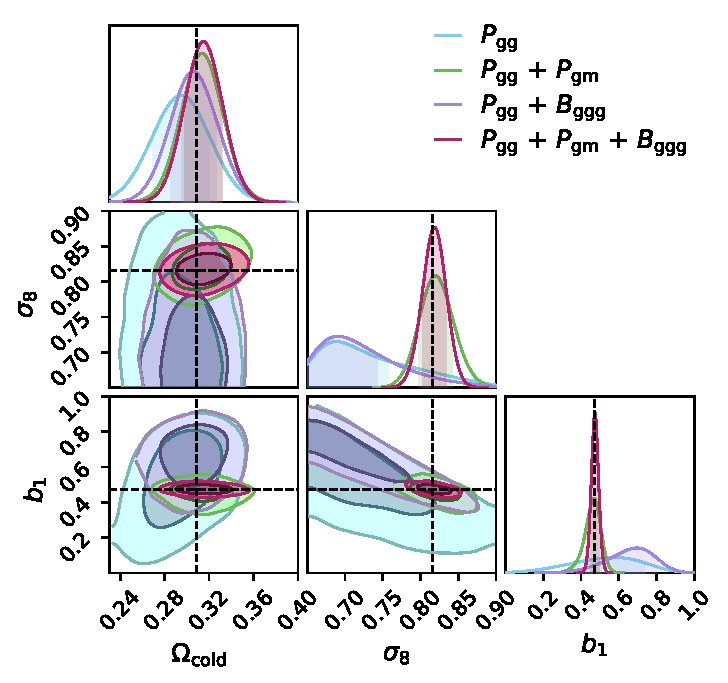
\includegraphics[width=\columnwidth]{figures/fig3_cosmic_variance_contours.pdf}
\caption{Posteriors for the key parameters $\om$, $\sig$, and $\bo$ inferred from the mean of the statistics over our cosmic variance test set, for each of the statistics combinations considered. The inclusion of $\pgm$ breaks the $\sig-\bo$ degeneracy, providing tight and unbiased constraints on the parameters; adding $\bispec$ tightens the constraints. The other bias parameters and the noise parameters are inferred and marginalized over; the full posterior plot is shown in Fig.~\ref{fig:cosmic_variance_full_posteriors}.}
\label{fig:cosmic_variance_contours}
\end{figure}

We find that we obtain tight, unbiased constraints on the cosmology and bias parameters when using the full combination of statistics ($\pk$ + $\pgm$ + $\bispec$), validating the inference approach.

While $\pk$ on its own provides significant constraining power on $\om$, it results in a weak constraint on $\bo$ and a weak, biased constraint on $\sig$. 
The weakness of these constraints is expected as a result of the perfect degeneracy between $\sig$ and $\bo$ in the power spectrum (as $\pk = (\bo\sig)^2 \hat{P}(k)$); we check that the combination $\sig\bo$ is accurately constrained.
Including $\bispec$ interestingly only slightly increases the precision on $\om$; further, it does not improve the bias on $\sig$.
Notably, it does signficantly increase the precision on the higher-order biases parameters $\bt$ and $\bs$. 
We see that using the statistics combination $\pk+\pgm$ produces unbiased constraints on $\sig$ and $\bo$; this makes sense as $\pgm$ is able to break this degeneracy (as $\pgm = \bo\sig^2 \hat{P}(k)$).
This corroborates our hypothesis that the bias observed in $\sig$ for $\pk$ and $\bispec$ is likely a result of projection effects caused by a lack of constraining power.
The full statistics combination $\pk$ + $\pgm$ + $\bispec$ preserves the unbiased constraints, and the bispectrum adds an additional improvement of constraining power compared to $\pk+\pgm$: it improves $\om$ by $\PrecPctCVMeanPkPgmBVsPkPgmOmegaC\%$, $\sig$ by $\PrecPctCVMeanPkPgmBVsPkPgmSigmaEight\%$, and $\bo$ by $\PrecFactorCVMeanPkPgmBVsPkPgmBo\times$, and notably the bias parameters $\bt$ by $\PrecFactorCVMeanPkPgmBVsPkPgmBt\times$, $\bs$ by $\PrecFactorCVMeanPkPgmBVsPkPgmBsTwo\times$, and $\bl$ by $\PrecFactorCVMeanPkPgmBVsPkPgmBL\times$.

We note that these results are for real space, and we would expect differences in the relative information content in the statistics in redshift-space, where there is additional cosmological information contained in redshift-space distortions.


\subsubsection{Coverage test set results}

We infer the parameters of the 1000 samples of our coverage test set, spanning the prior range of our training set; this allows us to test the dependence of the estimated parameters on the true parameter values.
Note that the prior has a wide range of values of the noise parameters, so these test samples will have a variety of noise levels.

\begin{figure*}
\centering
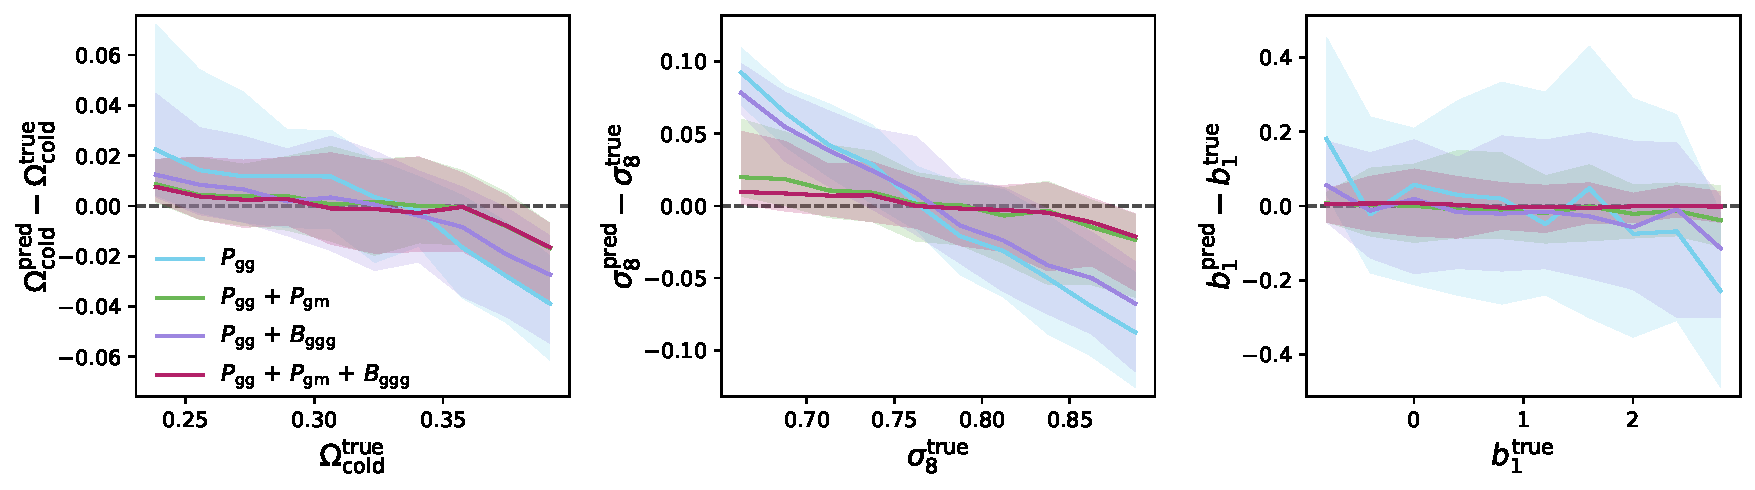
\includegraphics[width=\textwidth]{figures/fig4_coverage_binned_diff.pdf}
\caption{The difference between the predicted (mean of the posterior) and true parameter values for the key parameters for each of the 1000 coverage test set mocks, as a function of the true value. The median and 16th-84th percentile ranges in bins of the true value are shown for each of the stastistics combinations considered. Using the full statistics combination gives largely unbiased recovery across the prior range, with a small biases at the high ends of $\om$ and $\sig$; using fewer statistics results in stronger parameter-dependent biases that tend towards the mean. Including more statistics also results in tighter parameter constraints, most notably with $\pgm$ significantly improving the precision and bias on all key parameters.}
\label{fig:coverage_binned_diff}
\end{figure*}

In Figure~\ref{fig:coverage_binned_diff}, we show the differences between the predicted values and true values of the parameters as a function of the true value, which spans the full training prior; we display the median of the 1000 mocks, and the 16-84th percentile range.
The predicted value is the mean of the inferred posterior; we check that the behavior is very similar for the maximum a posteriori (MAP) values.
For $\pk$, we can see that the range of residuals is relatively wide, especially for $\bo$, and for all key parameters show a stronger bias with larger distance from the center of the prior.
This is expected when the statistic does not provide significant constraining power on the parameter, as is the case with $\pk$, as the prediction will tend towards the mean.
Including $\bispec$ improves the strength of the parameter-dependent bias for all parameters, and also generally tightens the range of the residuals.
When we consider $\pk+\pgm$, we can see that the bias on $\sig$ improves significantly, as $\pgm$ breaks the degeneracy with $\bo$ as we saw in the cosmic variance test set.
$\pgm$ also improves the constraints on $\om$ and $\bo$.
Further including $\bispec$ helps marginally, and this full parameter combination yields largely unbiased results across the coverage set, indicating that our inference is robust across the prior.
There are still slight biases for $\stats$ particularly at high $\om$ and $\sig$, so the analysis is most reliable towards the center of the prior.

\begin{figure*}
\centering
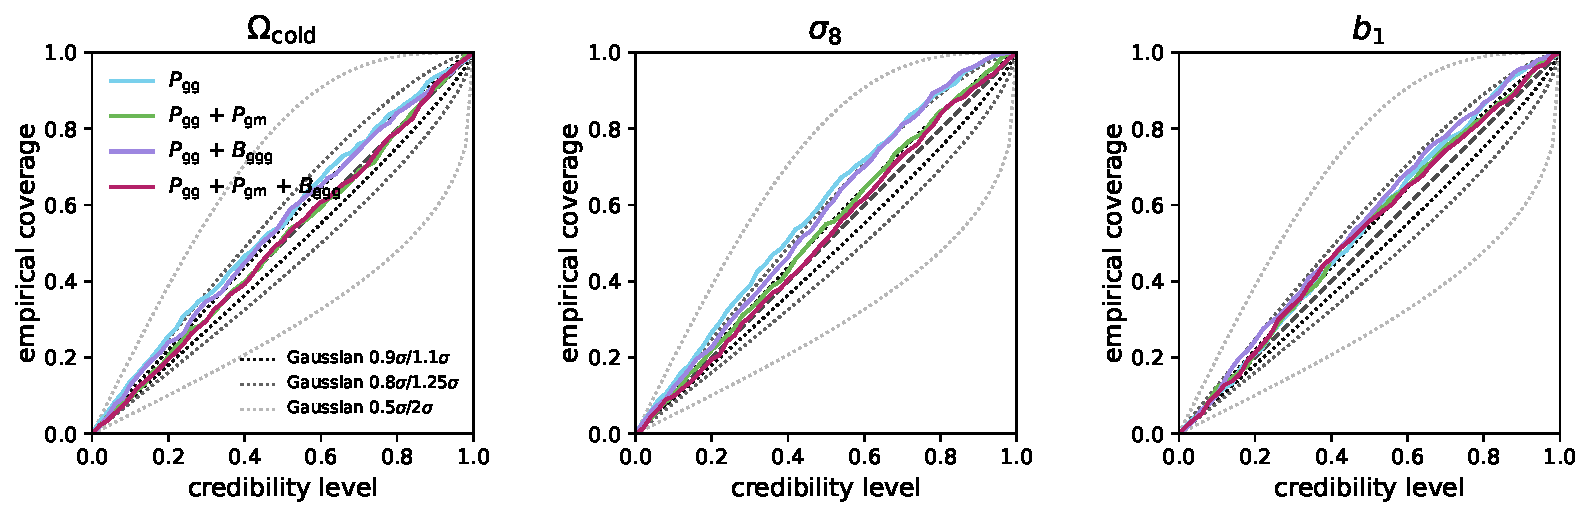
\includegraphics[width=\textwidth]{figures/fig5_coverage_pp_center500.pdf}
\caption{Coverage (probability--probability) plots for the key parameters for the 500 mocks of the coverage test set closest to the center of the prior. The empirical coverage is the fraction of test set points with predicted uncertainties at the given credibility level that encompass the true value. The closeness to the 1:1 line indicates well-calibrated uncertainties; dotted lines show the expected deviations if posterior widths were off by the given factor of $\sigma$, assuming Gaussians centered on the truth. The posteriors are largely well-calibrated, with the full statistics combination $\stats$ giving the best calibration across parameters.}
\label{fig:coverage_pp_center500}
\end{figure*}

The residuals shown above only quantify the accuracy of the means of the posteriors; to assess the inferred uncertainties, we compute the coverage of the samples, defined as the fraction of samples for which the true value falls within the predicted uncertainty range, as a function of the given level of uncertainty.
For instance, for a credibility level of 68\%, 68\% of the samples should have the truth fall within their predicted 68\% error region (``empirical coverage'').
A higher empirical coverage compared to credibility level indicates underconfidence, while lower indicates overconfidence.
This coverage (or probability-probability) plot is shown in Figure~\ref{fig:coverage_pp_center500}, for the 500 mocks of the coverage set closer to the center of the prior in $\om$, $\sig$, and $\om$.
We see that the inferred uncertainties are generally quite well calibrated for all three key parameters.
Using only $\pk$ or $\pk+\bispec$ results in a slight underconfidence in the posteriors, at the level of $0.1-0.25\sigma$ (assuming a Gaussian distribution centered on the truth).
The full statistics combination $\pk+\bispec+\pgm$ results in improved calibration of the uncertainties, with only slight fluctuations.
We note that for this check, we have excluded the mocks on the edges of the prior to isolate the assessment of the SBI-inferred uncertainties; when we make the coverage plot for all 1000 mocks of the coverage set, we do see some overconfidence.
This is a result of the biases towards the edges of the prior which cause the uncertainty regions to not sufficiently cover the truth, and the uncertainty estimates do not fully compensate for this bias.

These results show that our inference pipeline can accurately recover the cosmological and bias parameters across a range of parameter values.


\subsection{Out-of-distribution recovery test: SHAMe mock}

\begin{figure}
\centering
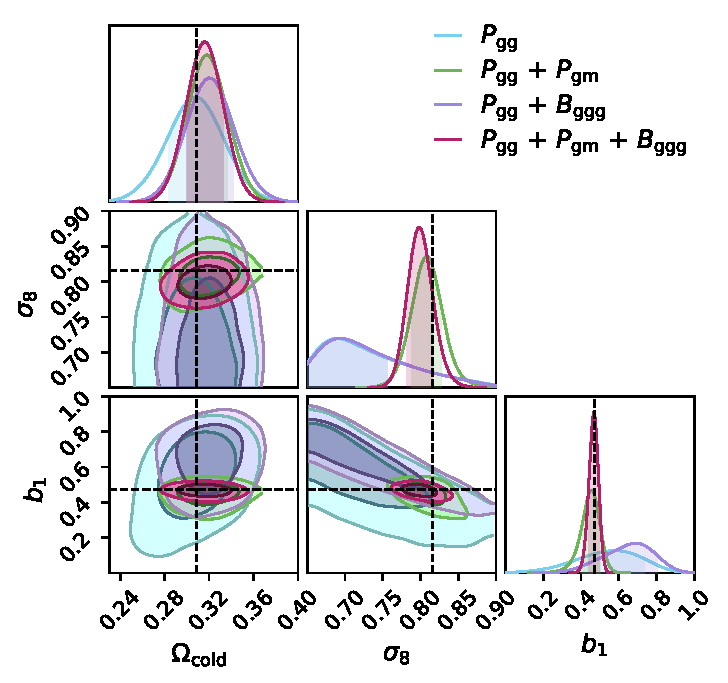
\includegraphics[width=\columnwidth]{figures/fig6_shame_contours.pdf}
\caption{Posteriors for the key parameters $\om$, $\sig$, and $\bo$ for our out-of-distribution SHAMe mock test, for each of the statistics combinations considered. The recovered parameters with the full statistics combination are unbiased within $1\sigma$, and the statistics show similar constraining power as in the in-distribution test. The full posterior plot is shown in Fig.~\ref{fig:shame_full_posteriors}.}
\label{fig:shame_contours}
\end{figure}

The results of our SBI pipeline on our SHAMe out-of-distribution test mock with fiducial number density $\nbarfid$ are shown in Figure~\ref{fig:shame_contours} for the key parameters (the full contours are shown in Figure~\ref{fig:shame_full_posteriors}).
We obtain generally unbiased constraints on the cosmological and bias parameters when using the full statistics combination, with $\om$, $\sig$, and $\bo$ all within $1\sigma$ from the true values.
The trends for the statistics generally follow those seen in the cosmic variance test set (\S\ref{sec:res_indist} and Figure~\ref{fig:cosmic_variance_contours}), with $\pgm$ breaking the degeneracy between $\sig$ and $\bo$, and $\bispec$ improving constraints significantly for the bias parameters and moderately for the cosmological parameters.
For the SHAMe data, we obtain a $\PrecPctShameOodFidPkPgmVsPkOmegaC\%$ improvement in precision on $\om$ and a $\PrecFactorShameOodFidPkPgmVsPkSigmaEight\times$ improvement on $\sig$ when including $\pgm$ compared to $\pk$ alone; additionally including $\bispec$ results in $\PrecPctShameOodFidPkPgmBVsPkPgmOmegaC\%$ and $\PrecPctShameOodFidPkPgmBVsPkPgmSigmaEight\%$ improvements on $\om$ and $\sig$ respectively compared to $\pk+\pgm$.

We do see moderate biases in the values of $\bt$ and $\bs$ when using the full statistics combination, at the \FoBSigmaShameOodFidPkPgmBBt$\sigma$ and \FoBSigmaShameOodFidPkPgmBBs$\sigma$ levels, while these were on average accurately constrainted in the cosmic variance test set.
This is likely a result of the bias parameters absorbing some model mismatch, which could be an issue for approaches such as imposing tighter priors on bias parameters; however, for our inference the cosmological parameters remain unbiased.

\begin{figure}
    \centering
    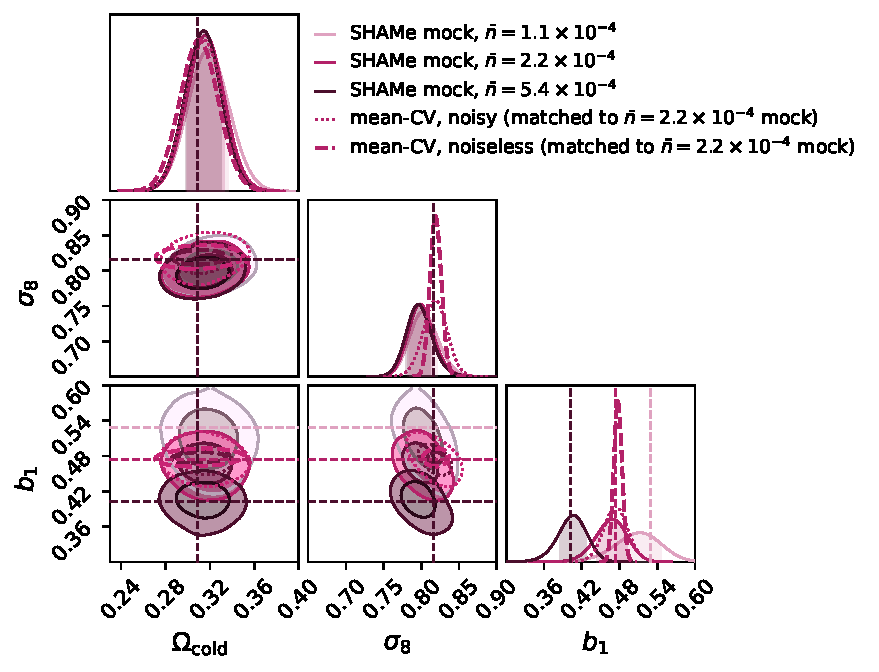
\includegraphics[width=\columnwidth]{figures/fig7_noise_impact_contours_nbars.pdf}
    \caption{Posteriors for $\pk+\bispec+\pgm$ for the key parameters, for varying number density and noise models. The filled contours show the results for the SHAMe OOD mock data with different number densities. The dotted contours show inference on the mean of the cosmic variance test set, which was matched to the fiducial $\nbarfid$ SHAMe mock; the dashed contour shows that same set but generated without any noise, and inferred assuming noiseless data.}
    \label{fig:noise_impact_contours_nbars}
    \end{figure}

We show the results for the full statistics combination $\stats$ on the SHAMe samples with a range of number densities in Figure~\ref{fig:noise_impact_contours_nbars}.
We find that the constraints on the cosmological parameters are robust to the noise level across this range.
The constraints on the bias parameter $\bo$ do lose precision at lower number densities; this could be related to degeneracies with the noise parameters.
We note that the noise parameters themselves are poorly constrained, as seen in the full contour plot (Figure~\ref{fig:shame_full_posteriors}).
However, we check that the noise model is necessary for properly inferring the parameters; assuming noiseless training data results in strong biases in the inference.

We also show the results for inference on the mean data vectors of the cosmic variance sample, which was generated with bias and noise parameters matched to the $\nbarfid$ SHAMe sample.
The precision of the predicted parameters is similar to that of the actual SHAMe sample, with somewhat tighter constraints for the in-distribution mock.
The bias in $\sig$ for the SHAMe mock disappears, indicating that the cause is model misspecification.
We additionally perform a test generating a cosmic variance test set with the SHAMe bias parameters but no noise, and then train the SBI model on noiseless training data. \ksf{check that this is properly described in the test set section}
We find that the constraints are consistent with the noisy case for $\om$, but improve signficantly for $\sig$ and $\bo$, demonstrating the constraining power lost to noise, even with perfect knowledge of the noise model.

These tests on out-of-distribution data demonstrates the generalizability of our forward model to realistic galaxy populations constructed with completely different underlying models.



\subsection{Scale dependence}

\begin{figure}
\centering
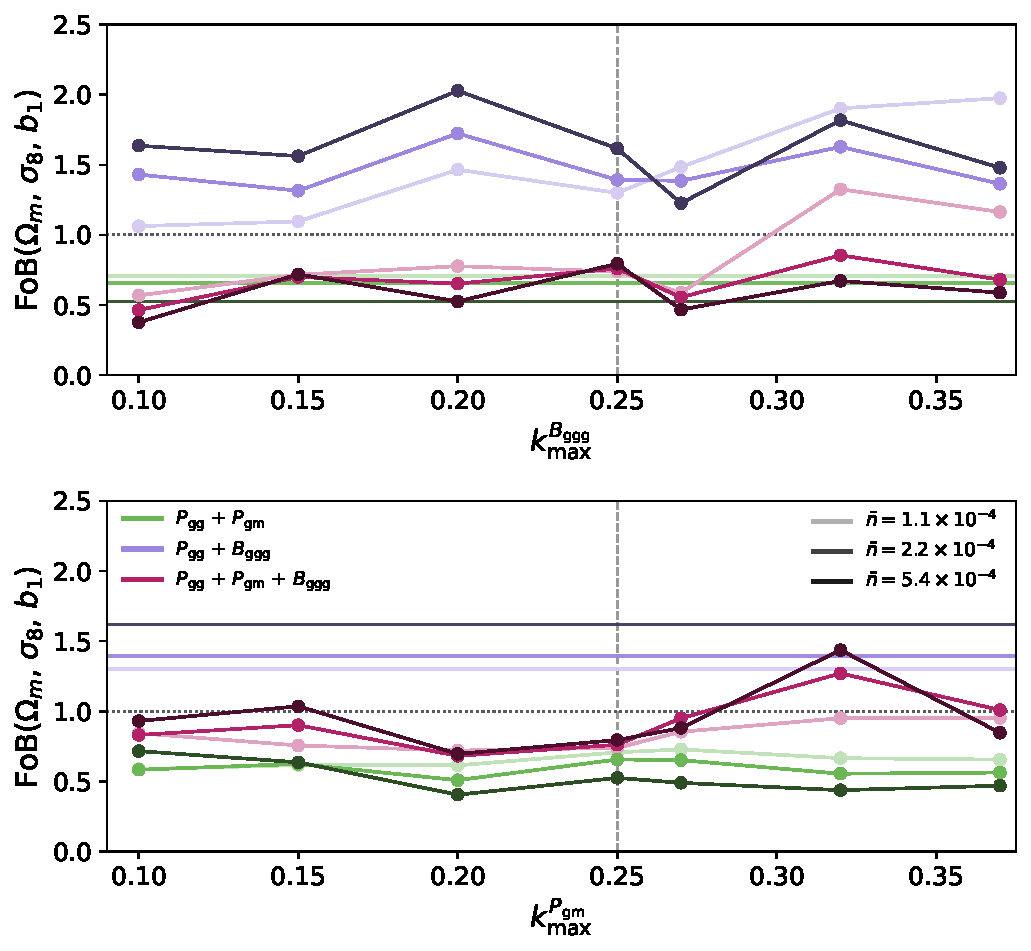
\includegraphics[width=\columnwidth]{figures/fig8_scale_dependence_fob3_nbars.pdf}
\caption{Scale dependence of the figure of bias (FoB) for the three key parameters combined for the SHAMe out-of-distribution mock, with varying number density. The top panel shows the FoB as a function of $\kmax$ for the bispectrum, fixing to our fiducial $\kmax=0.25$ for $\pgm$; the bottom panel shows it as a  function of $\kmax$ for $\pgm$, fixing to our fiducial $\kmax=0.25$ for the bispectrum. In both cases, the FoB for the full statistics combination remains around or below $1\sigma$ until $\kmax=0.25$, after which the inference becomes biased.}
% \ksf{slight bias for pgg+b coming from projection effects? could make this plot for cosmic variance set... maybe just mention that these are vol effects. or look at the params individually. incl b1 times sig8. could add a param orthogonal to that product; sigma8/b1.} \ksf{lowest 2 pink points on top plot confusing that they go above green points. look at contour plots} \ksf{maybe because noise model not affecting pgm!} \ksf{marcos: at low kmax end, looks like noise when still dominated by priors. noise parameters are close to edges?} \ksf{consistent with marcos's paper - with just pgg+bgg, no clear break. only when include matter.}
\label{fig:scale_dependence_fob3_nbars}
\end{figure}

We investigate the dependence of our results on the maximum $k$ scale included in our inference, for each of the statistics.
We keep the maximum scale for $\pk$ fixed to $\kmax=0.37\,\hMpc$, a bit below the Nyquist frequency of the box.
At this scale, the \mtm emulator of $N$-body displacements is shown to achieve significantly sub-percent accuracy ($\sim$0.2\%) on the power spectrum \citep{jamieson_field_2023}, and \cite{pellejero_ibanez_hybrid-bias_2023} showed that \mtm combined with the hybrid Lagrangian bias expansion to second order achieves 1-2\% precision to $\kmax=0.6\,\hMpc$.
(Previous works using the hybrid bias expansion with a power spectrum emulator find accuracy down to $\kmax=0.6\,\hMpc$ \citep{hadzhiyska_hefty_2021,zennaro_bacco_2023}.)
For the bispectrum, \cite{ibanez_validation_2026} recently validated the hybrid bias expansion down to $\kmax=0.25\,\hMpc$.
\ksf{anything to cite/mention for the cross-power-spectrum?}

In Figure~\ref{fig:scale_dependence_fob3_nbars}, we show the figure of bias for the SHAMe out-of-distribution mock for the three key parameters $\om$, $\sig$, and $\bo$ combined, as a function of the $\kmax$ of $\bispec$ and $\pgm$; when varying $\kmax^\mathrm{\bispecsh}$, we fix $\kmax^\mathrm{\pgmsh}=0.25\,\hMpc$, and when varying $\kmax^\mathrm{\pgmsh}=0.25\,\hMpc$ we fix $\kmax^\mathrm{\bispecsh}=0.25\,\hMpc$.
We see that using only $\pk+\bispec$ results in a bias moderately above $1\sigma$ for all number density samples, regardless of $\kmax$; this is likely largely a result of projection effects.
When including the cross spectrum, $\stats$, the inference is accurate to $1\sigma$ up until $\kmax^\mathrm{\bispecsh}=0.25\,\hMpc$, aligning with the result validating the hybrid bias expansion on the bispectrum and indicating that the limiting factor is the expansion rather than the emulated displacements.
The statistics combination $\pk+\pgm$ results in accurate inference for all number densities through $\kmax^\mathrm{\pgmsh}=0.37\,\hMpc$.
However, when additionally adding $\bispec$, the inference becomes biased pushing below $\kmax^\mathrm{\pgmsh}=0.25\,\hMpc$.
We also check the full grid of combinations, and find $\kmax^\mathrm{\bispecsh}=0.25\,\hMpc$, $\kmax^\mathrm{\pgmsh}=0.25\,\hMpc$ to be the optimal combination of limiting scales; pushing either or both to smaller scales results in further bias.
It is initially odd that pushing $\pgm$ to smaller scales results in a bias only when including the $\bispec$; we speculate that this could be because our noise model does not account for noise in $\pgm$, though further investigation is merited.

\begin{figure}
    \centering
    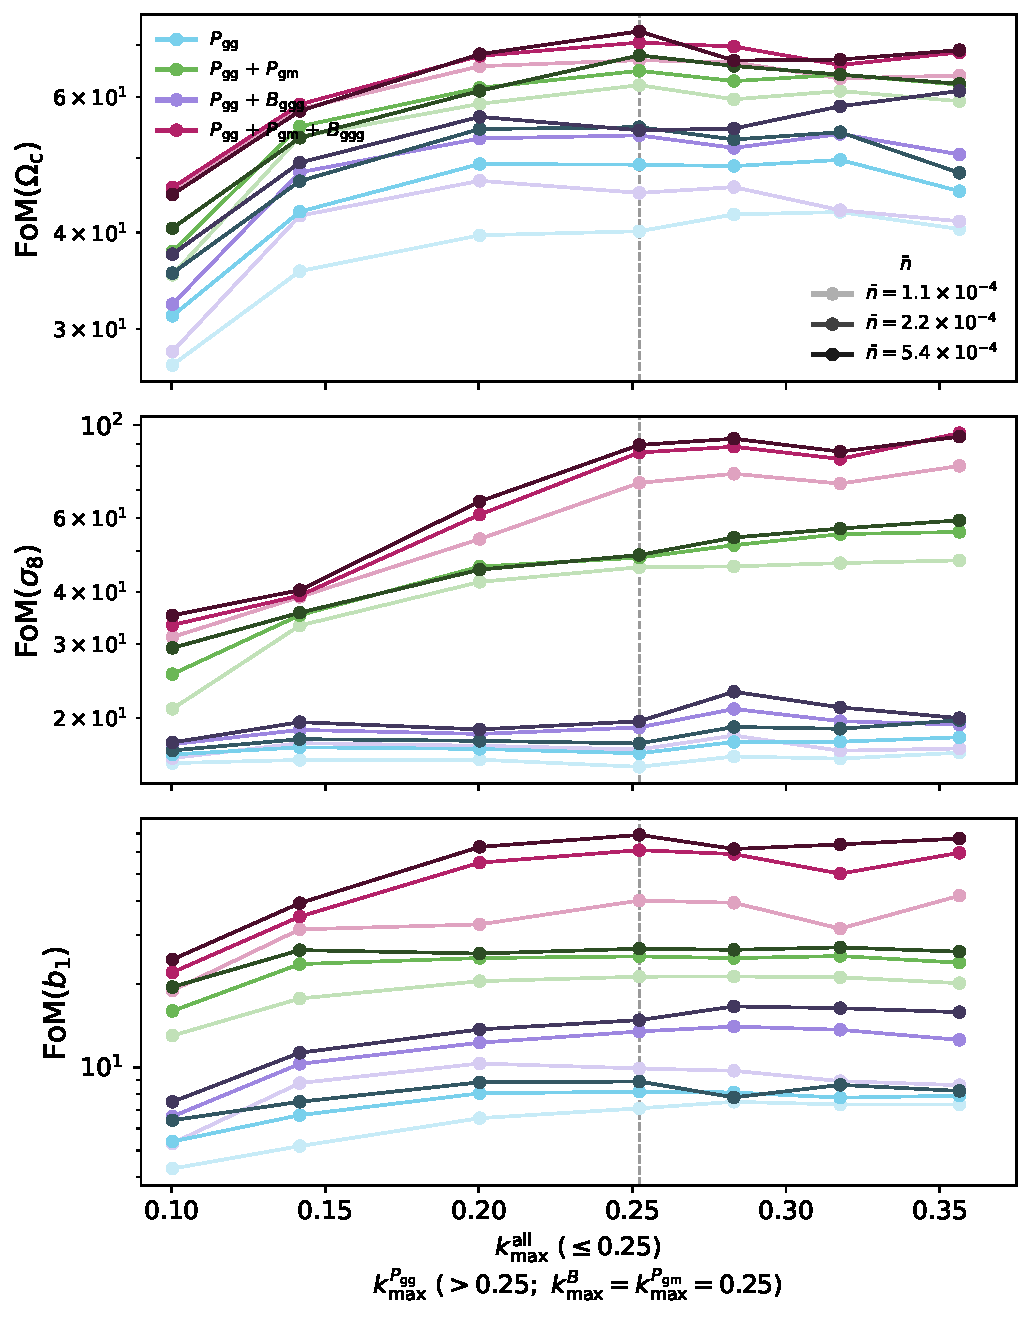
\includegraphics[width=\columnwidth]{figures/fig9_scale_dependence_fom_nbars.pdf}
    \caption{Scale dependence of the figure of merit (FoM) for the three key parameters for the SHAMe out-of-distribution mock, with varying number density. The $\kmax$ is for all three statistics for $k<0.25$; for $k>0.25$, we fix $\kmax^\mathrm{\pgmsh}=\kmax^\mathrm{\bispecsh}=0.25$ and only include higher $k$ for $\pgg$. Precision increases with scale, particularly for $\sig$ for $\stats$. \ksf{make legends, axis labels bigger}}
    \label{fig:scale_dependence_fom_nbars}
    \end{figure}

We explore the dependence of the figure of merit on the maximum scale included in the inference in Figure~\ref{fig:scale_dependence_fom_nbars}.
We show the FoM for the three key parameters for the SHAMe mocks at each of the three number densities tested, for all statistics combinations.
For $k<0.25$, we apply the same $\kmax$ for all three statistics; for $k>0.25$, we fix $\kmax^\mathrm{\pgmsh} = \kmax^\mathrm{\bispecsh}=0.25$ (the fiducial values chosen based on the FoB analysis above) and only include higher $k$ for $\pgg$.
We find that for nearly all the statistics combinations, parameters, and number densities, there is a significant increase in precision from $k=0.1$ to $k=0.25$.
The exception is $\pk$ alone for $\sig$; the information content is already saturated at larger scales.
Interestingly, there is not signficant information gain for most statistics combinations or parameters beyond $\kmax=0.25$, nor is there a clear trend with number density.
We find that the strongest increases in the FoM from $\kmax^\mathrm{all}=0.2$ to $\kmax^\mathrm{\pggsh}=0.37$ is for $\sig$ with $\pk+\pgm$ and $\stats$, increasing by $\FoMIncrPctShameOodFidPkPgmSigmaEightKmaxMaxVsKmaxEFT\%$ and $\FoMIncrPctShameOodFidPkPgmBSigmaEightKmaxMaxVsKmaxEFT\%$ for $\nbarfid$.
These are quite significant gains; this demonstrates the value of using the hybrid bias expansion approach in comparison to EFT approaches, which are limited to $k=\sim$$0.1-0.2$.


\subsection{Dependence on number of cosmologies and bias parameter sets}

We explore the convergence of our inference with the number of training data points.
We vary the number of cosmologies by selecting only a subset of cosmologies to train the network with, choosing $N_\mathrm{cosmo}=500,1000,2000,4000,6000,8000,10000$; the subsets are nested to minimize random variance.
To vary the number of bias parameters, we train on each layer of the nested Latin hypercube of bias and noise parameters, resulting in a range of bias parameters per cosmology: $N_\mathrm{bias}=1,2,4,8,16,32$. 
For each of these combinations of the number of cosmology and bias parameters, we train a new model using the fiducial hyperparameters for the given statistics combination, and perform inference on the 1000 mocks of the coverage set.

\begin{figure}
\centering
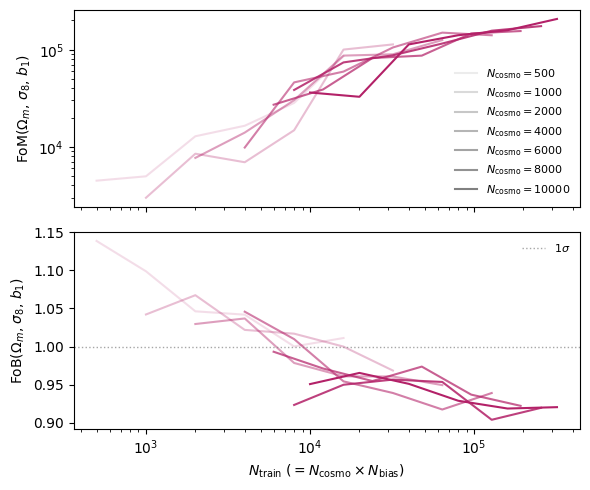
\includegraphics[width=\columnwidth]{figures/fig10_convergence_pgg_b_pgm.png}
\caption{Convergence of the inference with training set size, for $\pk+\bispec+\pgm$ on the coverage test set for the three key parameters $\om$, $\sig$, and $\bo$ combined. The top panel shows the figure of merit (FoM), and the bottom panel shows the figure of bias (FoB), normalized by the 68th percentile of the $\chi^2$ distribution for three dimensions (corresponding to the three parameters); the median values over the coverage set are shown. The opacity indicates the number of training cosmologies. Increasing the number of training points increases the precision signficantly until $N_\text{train}=\,\sim$20,000 and then more marginally, with the number of cosmologies and bias parameter sets contributing similar precision; the bias also plateaus around $N_\text{train}=\,\sim$20,000, with the number of cosmologies mattering more than the number of bias parameters for smaller $N_\text{train}$. \ksf{make legends, axis labels bigger} \ksf{note: this plot is with an older base model, with kmax=0.4 and no ensembling; running the new version right now}}
\label{fig:convergence_pgg_b_pgm}
\end{figure}

\begin{figure*}
\centering
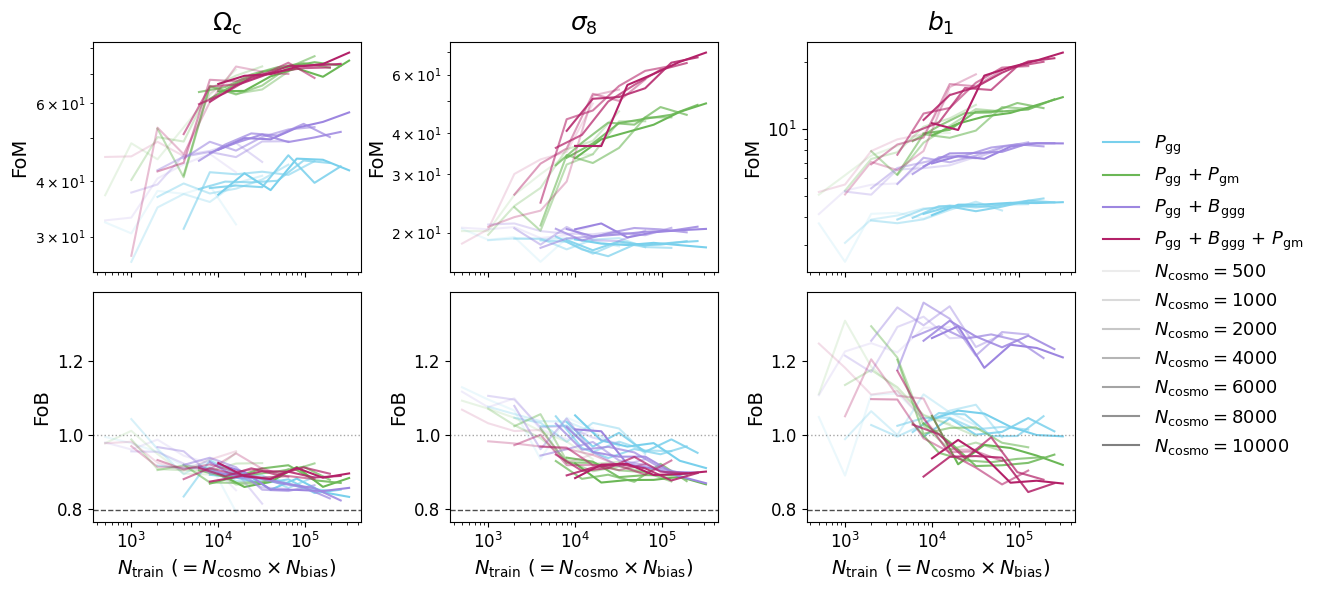
\includegraphics[width=\textwidth]{figures/fig11_convergence_all_combos.png}
\caption{Convergence of the inference with training set size, for all the statistics combinations on the coverage test set for the three key parameters $\om$, $\sig$, and $\bo$ individually. The top row shows the figure of merit (FoM) and the bottom row shows the figure of bias (FoB); the median values over the coverage set are shown. The opacity indicates the number of training cosmologies, and the dashed line indicates the expectation for an unbiased Gaussian distribution. The FoM increases with training set size for most statistics and parameters, with the exception of $\sig$ with $\pk$ and $\pk+\bispec$ which do not show improvement; all have an FoB around or below $1\sigma$. \ksf{note: this plot is with an older base model, with kmax=0.4 and no ensembling; running the new version right now}}
%  \ksf{not reaching 0.8 because network not good enough? non-gaussian?} \ksf{try with cosmic variance set?} \ksf{reach theory floor bc have addl source of noise; network + data vector, projection effects} \ksf{om probs comes mostly for geometric aspects of power spec (??)} \ksf{takeaway is that many are still not  converged. ref how many sims paper - but diff research question, number for emulator vs sbi?}
\label{fig:convergence_all_combos}
\end{figure*}

To assess the accuracy of our results, we use the figure of bias, defined as
\begin{equation}
    \mathrm{FoB} = \frac{1}{\chi^2_\mathrm{lim}} \sqrt{(\bm{\hat{\theta}} - \bm{\theta}_\mathrm{true})^T \mathcal{C}^{-1} (\bm{\hat{\theta}} - \bm{\theta}_\mathrm{true})} ~,
\end{equation}
where $\bm{\hat{\theta}}$ are the predicted values of the parameters, $\bm{\theta}_\mathrm{true}$ are the true values, and $\mathcal{C}$ is the covariance matrix, which is estimated from the posterior samples.
The quantity $\chi^2_\mathrm{lim}$ scales the FoB by the expected $\chi^2$ for the relevant number of dimensions and $\sigma$ value.
The $1\sigma$ expectation for three dimensions is $\chi^2_{\nu=3}(0.68)\approx1.88$, which we use for the parameter subspace $(\om, \sig, \bo)$; in this case we also compute $\mathcal{C}$ only across this subspace.
For one dimension this becomes $\chi^2_{\nu=1}(0.68)=1$, which reduces to the absolute error in terms of the standard deviation, $\mathrm{FoB}_\mathrm{1D} = |\hat{\theta} - \theta_\mathrm{true}|/\sigma_\theta$.

To assess the precision, we use the figure of merit (FoM), defined as
\begin{equation}
    \mathrm{FoM} = \frac{1}{\sqrt{\mathrm{det}\mathcal{C}}} ~,
\end{equation}
which is the inverse of the volume of the allowed region, meaning that a higher FoM indicates tighter constraints. 
Again we compute $\mathcal{C}$ only across the subspace considered; in one dimension, this reduces to $\mathrm{FoM}_\mathrm{1D} = 1/\sigma_\theta$.

Figure~\ref{fig:convergence_pgg_b_pgm} shows the figure of merit and figure of bias for the three key parameters combined, averaged over the coverage set, for the full statistics combination as a function of the total number of training points $N_\mathrm{cosmo} \times N_\mathrm{bias}$, shown as separate lines for each choice of $N_\mathrm{cosmo}$.
We see that the FoM increases with increasing number of training points, steeply until $N_\mathrm{train}=10,000$ and then more moderately. 
The FoM does not plateau even at $320,000$ training points, indicating that the inference is still not converged and the precision would continue to improve with additional training data.
The FoB similarly reduces sharply until $N_\mathrm{train}=10,000$ where it crosses $FoB=1\sigma$, but then more-or-less plateaus, indicating that above a few tens of thousands of training points, the training data is sufficient for unbiased inference.

We also find that there is not a strong trend with the number of training cosmologies, as shown by the lines for the different cosmologies largely overlapping.
With a smaller number of training data points (below $N_\mathrm{train}=20,000$), it is more important to have more cosmologies rather than more bias parameter sets, shown by the spread in the FoB around that value; however, beyond $N_\mathrm{cosmo}=2000$, it is sufficient to add more bias parameter sets per cosmology.
This somewhat surprising finding is encouraging given that generating training data at varying cosmologies is more expensive than populating each cosmology with varying bias parameter sets.
Previous SBI analyses already use around this number of training cosmologies with full $N$-body codes (without the need for emulators, e.g. the Quijote Latin hypercube); our result shows that this may be sufficient in terms of cosmologies, but that additional constraining power and robustness could be gained by populating these with many more galaxy formation parameter sets per cosmology.

In Figure~\ref{fig:convergence_all_combos}, we show the FoM and FoB for all the statistics combinations, for each key parameter individually.
Note that for a Gaussian sample, we would expect $FoB\approx0.8$; our FoB stays slightly higher than this for all the parameters, bottoming out at 0.85-1.0, possibly as a result of non-Gaussian behavior.
We see that for $\sig$, a small number of training cosmologies already saturates the precision for $\pk$ and $\pk+\bispec$, though around $N_\mathrm{train}=20,000$ are needed to reach a plateau in the FoB below $1\sigma$.
Similarly for $\bo$ for those statistics combinations, the precision begins to plateau around the same number of training points, and seems to saturate around $N_\mathrm{train}=100,000$.
The statistics combinations $\pk+\pgm$ and $\stats$ show steep improvements in both precision and accuracy until $N_\mathrm{train}=10,000$ for all parameters, and then improve more moderately.
Notably, by our maximum number of training points $N_\mathrm{train}=320,000$, the FoM has not yet plateaued, indicating that additional training data may continue to improve the inference and we have not yet extracted the full information content the statistics.
We also again find that for all parameters, increasing the number of bias parameter sets per cosmology results in similar FoM and FoB values as increasing the number of cosmologies, beyond a few thousand cosmologies.


\section{Discussion}
\label{sec:discussion}

The results of this analysis outline the successes and challenges of SBI with the hybrid Lagrangian bias expansion and emulated $N$-body displacements.
While we showed that our model is able to provide robust inference on cosmology, model extensions and adjacent analyses will add to our understanding of the information content in galaxy clustering and optimal approaches to extract it.

We have used Lagrangian bias expansion to second order; it is possible that extending into the third order may be necessary for more accurate modeling in the small-scale regime \ksf{citation for this / more to say?}.
For the stochastic noise, we have used a noise model based on a Gaussian field coupled to the bias fields following \cite{rubira_non-gaussian_2025}, to first order in the noise field. 
This is a more sophisticated model than a standard Gaussian field, or parametric noise models specific to each statistic; however, this still does not capture the noise in $\pgm$ and may not be suffient for other high-order statistics. 
Extending this noise model to higher order (at the expense of adding additional parameters) or testing other noise models may be important for ensuring the most robust inference.

While the \mtm emulator is shown to be accurate for the galaxy--galaxy power spectrum down to small-$k$, there are remaining issues for using it for csomological inference.
\cite{pellejero_ibanez_hybrid-bias_2023} found that when employing it for the hybrid bias expansion, there were biases at intermediate scales; while these were absorbed by noise nuisance parameters, inference could be sensitive to this depending on other modeling choices.
The emulator also has not been robustly validated for the whole range of higher order statistics or the full tracer field.
Improving the displacement emulator or further validating it will be key for future analyses.

\cite{bairagi_how_2025} explored the question of the required number of simulations for cosmological inference, using a large suite of 32,768 $N$-body simulations called the Big Sobol Sequence. 
Using neural posterior estimation on the nonlinear dark matter power spectrum down to $\kmax=0.8$, they found that around 4,000 simulations were required to saturate the information content, signifcantly more than the 2,000-simulation Quijote suite.
This stands somewhat in contrast to our finding, that on the one hand 2,000 cosmologies provide comparable results to 10,000 given an equal total number of simulations (including multiple galaxy bias parameter sets), and on the other even 320,000 total training data points does not seem to saturate in precision.
However, our convergence findings are not directly comparable, as their work analyzes a matter field statistic and does not sample galaxy bias parameters, so we would expect that fewer simulations are needed.
\cite{tucci_eftoflss_2024} also analyze the convergence of their EFT-based SBI approach with the number of simulations, finding that at fixed cosmology $10^5$ simulations are required to converge in the inference of the bias parameters.
In the free-cosmology case with one cosmological parameter, the inference is slower to converge, and is not clearly fully converged at their maximum $5\times10^5$ simulations; this is in line with our results that upwards of $10^5$ simulations are required for convergence.
Further work with large simulation suites in various regimes and different modeling choices is necessary to provide a complete picture of the convergence with the number of simulations.

The \mmocks approach has the potential to be expanded to answer further questions about the information content in galaxy clustering and the requirements for SBI.
With the $N$-body emulator costing only minutes and the summation of the bias fields with a choice of bias parameters being nearly instantaneous, even more mocks could be generated to understand where the information in various statistics saturates, as we found that some continue to rise with our full 320,000-mock suite.
We could also straightforwardly generate larger volumes with this approach, as current survey volumes are easily outpacing our ability to model these volumes with traditional simulations.
With modifications to the forward model, beyond-$\Lambda$CDM cosmologies could be explored to understand the sensitivity of various statistics to alternative cosmological models.

A key potential extension is to explore other statistics of the tracer fields to understand their information content.
Optimal summary statistics that capture the information content of the full field could be learned, to explore the maximal information in cosmological fields.
As we also forward model the velocity fields, this suite could be useful for exploring velocity reconstruction approaches.
One could also investigate the effect of more restrictive priors on the Lagrangian bias parameters, encoding our knowledge specific galaxy samples.

The SBI approach with the \mmocks model that we have demonstrated could be applied to more realistic data, and eventually to real data to perform a cosmological analysis.
This analysis has been entirely in real-space, and a redshift-space analysis is forthcoming.
Survey realism, including systematics, could be applied to the fields to understand the information content in more realistic settings. 
Finally, an analysis on survey data such as BOSS or DESI has the potential to provide competitive and complementary results.


\section{Summary and Conclusions}
\label{sec:conclusions}

In this work, we have presented a forward model for galaxy tracer fields that balances robustness and speed, and is useful for simulation-based inference approaches to cosmological inference.
The model uses the hybrid Lagrangian bias expansion to second order, based on emulated particle and velocity displacement fields from the \mtm emulator of \cite{jamieson_field_2023} trained on the Quijote mocks, to generate sets of bias fields that can be weighted and summed to produce tracer fields.
We also include a full-field noise model of \cite{rubira_non-gaussian_2025} based on a Gaussian field coupled to the bias fields, which we find to be critical for unbiased inference.
With this forward model, a $(1 \Gpch)^3$ mock can be generated at any cosmology in around 8 minutes. 
We publicly release a suite of these bias fields,  called \mmocks, at $z=0$ in both real- and redshift-space.
Our main mock set consists of a Latin hypercube of 10,000 different cosmologies; we also release an independent 1,000-cosmology Latin hypercube ``coverage'' test set, and a 1,000-realizations ``cosmic variance'' set at fixed cosmology with varying seeds.

We perform simulation-based inference using use neural posterior estimation.
We generate training data from our forward model, recombining each bias field set at a given cosmology with up to 32 bias and noise parameter sets, for a total of 320,000 traning mocks.
The summary statistics considered are the galaxy--galaxy power spectrum $\pk$, the galaxy--matter cross-spectrum $\pgm$, and the galaxy bispectrum $\bispec$.
In addition to the in-distribution tests sets described above, we apply our model to a realistic out-of-distribution mock built with the extended Subhalo Abundance Matching (SHAMe) model on a high-resolution \bacco simulation.
With this approach, our findings are the following:
\begin{itemize}
    \item Inference with $\pk$ alone suffers from strong projection effects, resulting in biased $\sig$ even for the in-distribution test sets; this holds even when additionally including $\bispec$. Including $\pgm$, which is related to the  galaxy--galaxy lensing observable, results in unbiased inference of $\om$, $\sig$, and $\bo$, as it breaks parameter degeneries and ameliorates projection effects (see Figs. \ref{fig:cosmic_variance_contours} and \ref{fig:coverage_binned_diff}).
    \item We recover unbiased cosmological parameters on the out-of-distribution SHAMe mock, validating the robustness of our model. This holds down to scales of $\kmax=0.35$ for the galaxy--galaxy power spectrum, and $\kmax=0.25$ for the galaxy--matter cross spectrum and the galaxy bispectrum (see Figs. \ref{fig:shame_contours} and \ref{fig:scale_dependence_fob3_nbars}).
    \item Increasing the number of bias parameter sets applied to each cosmology achieves a similar precision and accuracy as increasing the number of cosmologies, for the same total number of points, beyond a minimum of around 2,000 cosmologies (see Fig. \ref{fig:convergence_all_combos}). This could be a very helpful result, as augmenting with more galaxy bias combinations is far faster than generating mocks at new cosmologies.
    \item For $\pk$ alone, around 20,000 training mocks are required for inference to converge and information content to saturate; for the full statistics combination $\stats$, the precision continues to increase even with 320,000 training points, indicating that additional mocks (or improved SBI procedures) are needed to saturate the information in those statistics (see Fig. \ref{fig:convergence_pgg_b_pgm}).
\end{itemize}

The \mmocks suite will be publicly available, and is useful for various analyses exploring the information content in galaxy clustering.
With its large number of mocks and robust method for modeling the galaxy--dark matter connection, it is ideal for testing approaches to simulation-based inference.
The approach could be extended to generate mocks exploring a range of science questions and targeted for specific tracer populations and surveys, paving the way for robust and flexible inference from galaxy clustering.


\section*{Acknowledgements}

The authors would like to thank Beatriz Tucci, Ivana Nikolac, Matt Ho, and Jed Homer; Matteo Zennaro, Daniel L\'opez-Cano, Francisco Maion and the rest of the \bacco group; and Risa Wechsler and the KIPAC Galaxy Formation and Cosmology group for helpful discussions.

\section*{Software and LLM Usage}

The following software were used in this work: \ksf{fill in software}
In this work, large language models (LLMs) were used to make code modifications, write basic code such as plotting functions, support background research, and provide basic \LaTeX support.
Core code and all writing did not involve the use of LLMs.

\section*{Data Availability}

The \mmocks suite and the code used in this paper will be made publicly available at \url{this url}.

%%%%%%%%%%%%%%%%%%%% REFERENCES %%%%%%%%%%%%%%%%%%

\FloatBarrier
\clearpage
\bibliographystyle{mnras}
\bibliography{references,references_extra}

%%%%%%%%%%%%%%%%%%%%%%%%%%%%%%%%%%%%%%%%%%%%%%%%%%

%%%%%%%%%%%%%%%%% APPENDICES %%%%%%%%%%%%%%%%%%%%%

\appendix

\section{Validation of inference on mean data vector}
\label{sec:meandemo}

\begin{figure}
\centering
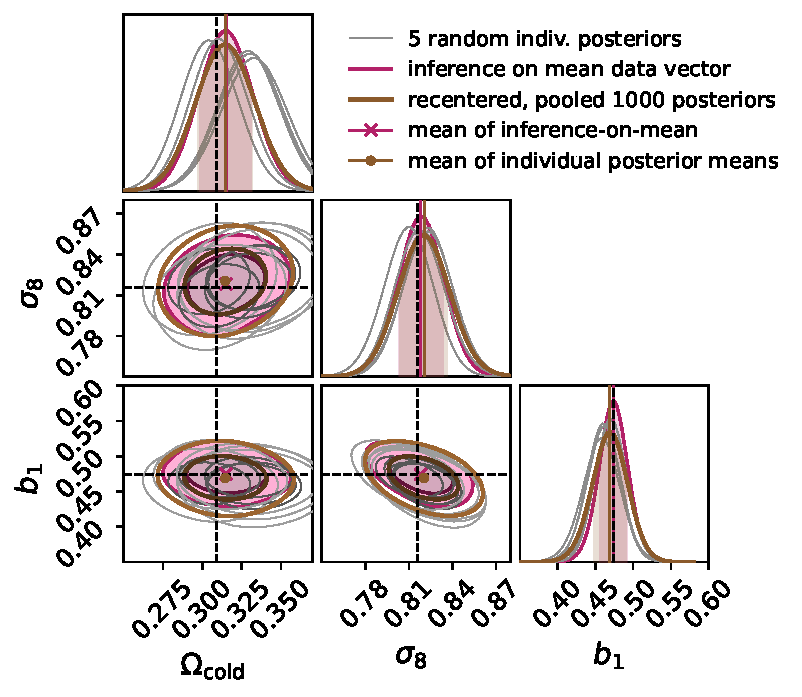
\includegraphics[width=\columnwidth]{figures/figA_mean_vs_indiv_means_contours.pdf}
\caption{Validation of inference on the mean of the data vectors for the cosmic variance test set, for the full $\pk+\bispec+\pgm$ combination. The grey contours show posteriors from inference performed on statistics of 5 randomly selected realizations from the test set; the brown contours are pooled samples from each of the 1000 realizations, 500 of each recentered to the mean of the means; the magenta contours show inference performed on the mean of 1000 data vectors. The mean of the inference-on-the-mean (magenta vertical line and X marker) nearly exactly agrees with the mean of the 1000 individual posterior means (brown vertical line and dot marker). The shape and width of the posteriors are also broadly consistent.}
%\ksf{bc network is focusing on low dim representation} \ksf{in each projection, get peak of dist (or mean); and plot 2d hist of the grey means. and the 1ds, will be a hist of grey vs the contours} \ksf{dont need to focus on uncertainties} \ksf{importance sampling of the posteriors of individuals - interpolate to get posterior value for each point in param space. then could combine. can share data with marcos} \ksf{test with fewer than 1000 to see if an issue with number of points}
\label{fig:mean_vs_indiv_means_contours}
\end{figure}

In this analysis, we have shown results of the SBI pipeline with the \mmocks forward model on the ``cosmic variance'' test set, which contains 1000 realizations run with different seeds at the same cosmology, bias, and noise parameters.
Specifically, we took the mean of the 1000 data vectors computed on each of these mocks individually, and used that mean data vector as the input to the SBI model.
In this section, we investigate this analysis choice and its implications.

% To understand the result of this inference on the mean data vector (``inference-on-the-mean''), we also perform the inference on each of the 1000 mock realizations individually and obtain posteriors for each.

We first compute the statistics on all 1000 mock realizations, and perform the inference on each individually with our SBI pipeline.
We obtain a posterior for each of the 1000 realizations.
To visualize the ``typical'' posterior, we compute the mean-of-the-means of the 10000 posteriors, and shift each posterior such that it is centered on that value; we then pool the posteriors, drawing 500 samples from each.

We then compute the mean of the statistics of the 1000 mocks, and perform the inference on that mean data vector.
This mean data vector has the benefit of reducing the effect of cosmic variance on the statistic, but brings the complication of having a different covariance than the data the SBI model was trained on (namely, much lower variance).
In standard MCMC approaches, this would be handled by appropriately scaling the covariance matrix, but in the context of SBI, the covariance is learned by the model from the training data and is not given explicitly.
Thus it is important to understand the behavior of the model when we use the mean data vector for inference.

Figure~\ref{fig:mean_vs_indiv_means_contours} shows the result of these ways of analyzing the cosmic variance test set, all for the combined statistic $\stats$.
The grey contours show posteriors of 10 randomly selected individual mocks; the brown contour shows the recentered-pooled posteriors (over all 1000 mocks); and the magenta contour shows the inference performed on the mean of the 1000 data vectors.
The brown dot and vertical lines show the mean of the means of the 1000 individual posteriors.

We see that the inference on the mean produces a posterior very close to that of the recentered-pooled posterior.
The means, as well as the MAPs, for these two results are within $\sim$1\% for all parameters; both are within $0.5\sigma$ (2\%) from the true values.
The predicted uncertainty regions are also very similar: the symmetrized inner 68\% width agrees to $\FracDiffPctErrCVRecenteredVsCVMeanPkPgmBOmegaC\%$ for $\om$, $\FracDiffPctErrCVRecenteredVsCVMeanPkPgmBSigmaEight\%$ for $\sig$, and $\FracDiffPctErrCVRecenteredVsCVMeanPkPgmBBo\%$ for $\bo$.
We check that the recentered-pooled posterior width agrees with the mean of the widths of the 1000 individual posteriors, to better than 0.5\%.
The inference-on-the-mean does generally produce slightly tighter constraints than the average of the individual posteriors, interpreted as mild overconfidence.
However, the mean data vector should be less affected by prior effects than individual realizations with summary statistics towards the edges of the distribution.
\ksf{i think we still don't know exactly how to interpret this; so i am not sure how to tie these last couple sentences together.}

This analysis indicates that despite the lower variance of the mean data vector, the SBI pipeline produces a posterior that has the typical width of a posterior estimated with the noisier data vector, as that was closer to the noise levels of data it was trained on.
We thus use the inference on the mean data vector throughout the paper to be able to show the typical result of the inference, with the effect of cosmic variance (which would cause a bias in any given individual sample) removed.
We emphasize that there is not a clear statistical interpretation of this inference-on-the-mean for simulation-based inference, and the stability of the comparison to the individual posteriors varies somewhat across models.
However, the results empirically demonstrate that this is a useful way to validate an SBI pipeline with a much lower computational burden compared to sampling many individual posteriors.



%%%%%%

%\ksf{i am not quite sure how to square the results of the number density plot with the mean-on-inf comparison. when we perform inference on the mean of 1000, we get the same posterior size as any individual. but when we use the higher number density shame model, we do get a smaller posterior size compared to the lower number density one. (i think the noiseless one makes a bit more sense, as that's actually a different model where we also train on noiseless data. but the different noise levels of shame are all using the same model with the same training data.)}



\section{Full posterior contours}

\begin{figure*}
\centering
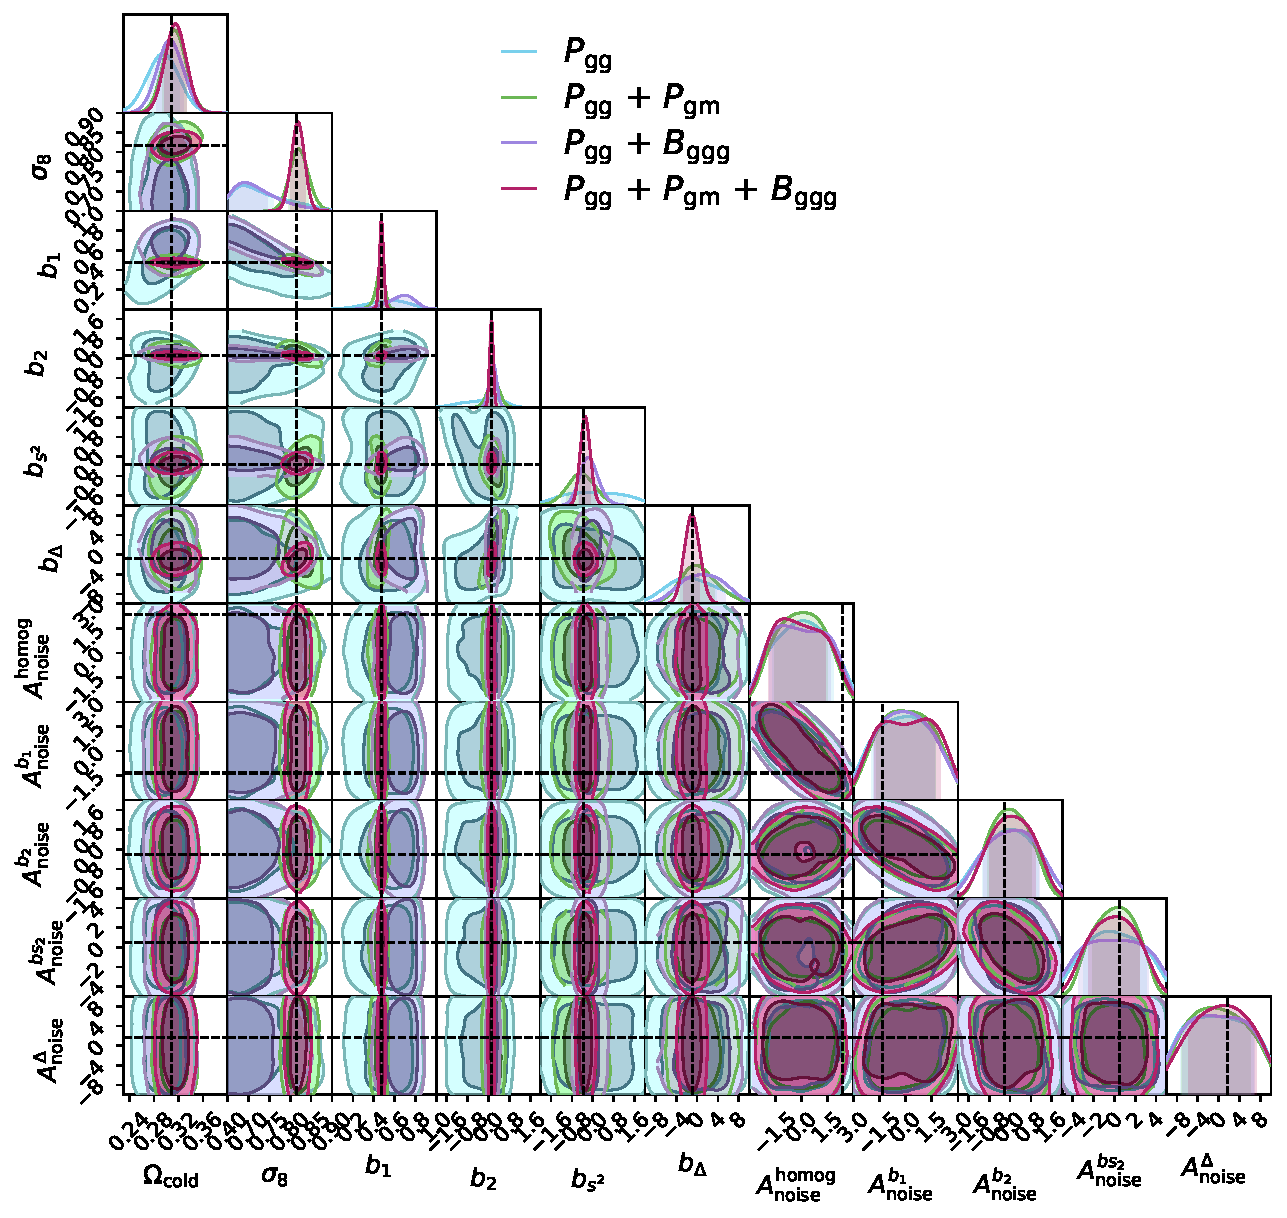
\includegraphics[width=\textwidth]{figures/figB1_cosmic_variance_full_posteriors.pdf}
\caption{Full posterior contours for the cosmic variance test set.}
\label{fig:cosmic_variance_full_posteriors}
\end{figure*}

\begin{figure*}
\centering
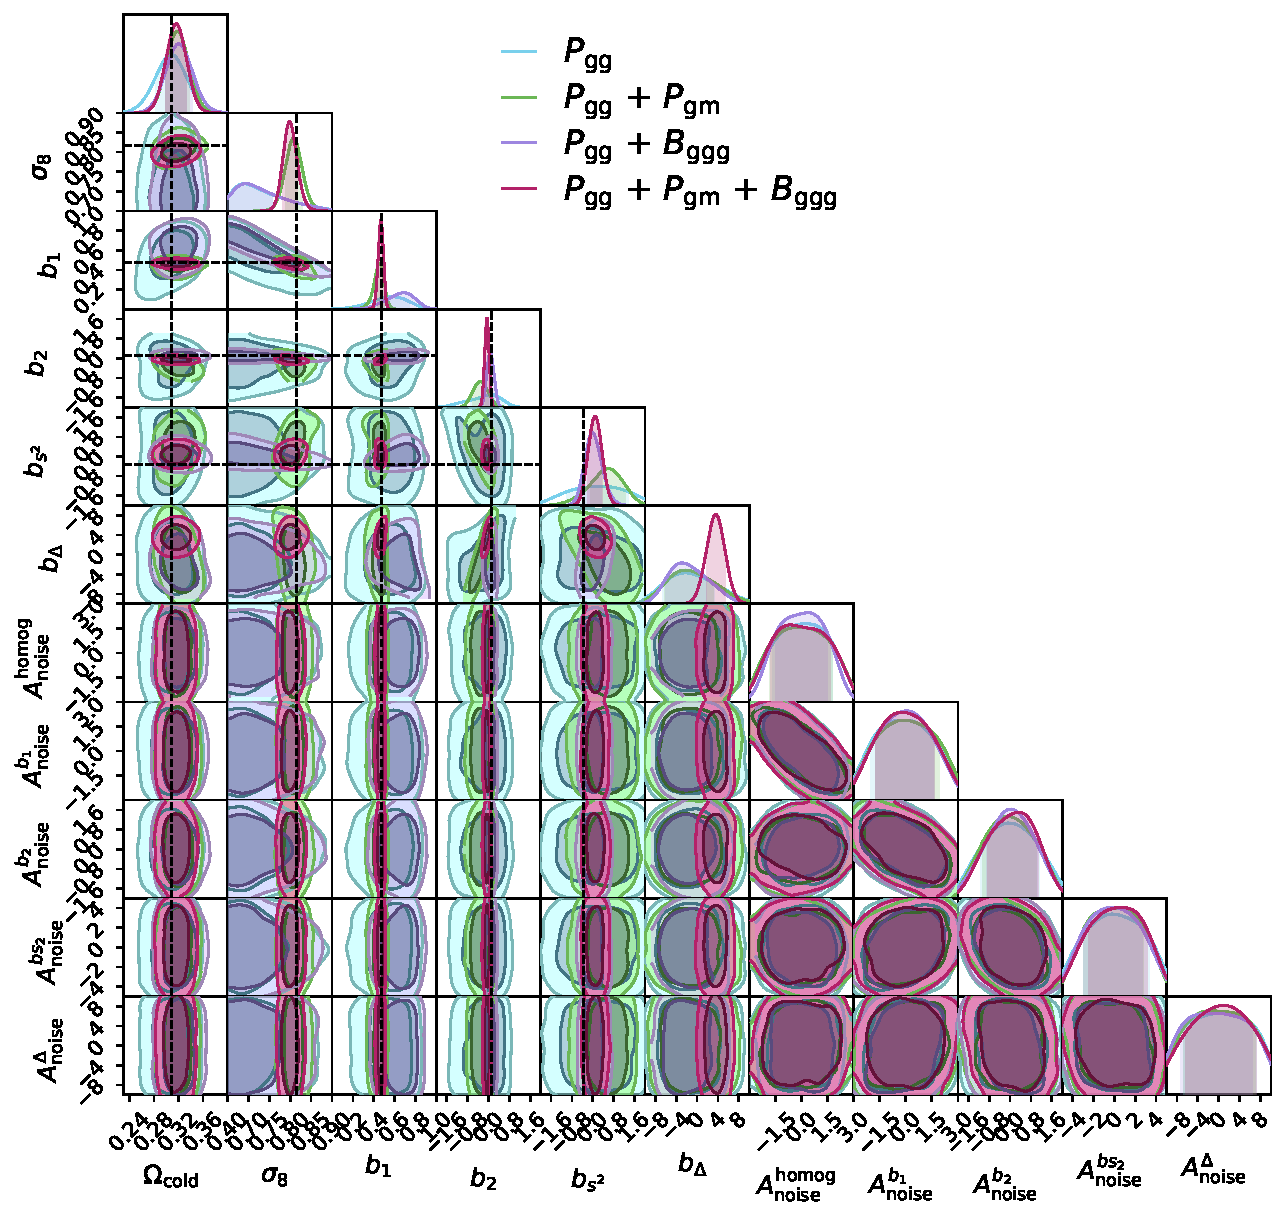
\includegraphics[width=\textwidth]{figures/figB2_shame_full_posteriors.pdf}
\caption{Full posterior contours for the SHAMe test set.}
\label{fig:shame_full_posteriors}
\end{figure*}

%%%%%%%%%%%%%%%%%%%%%%%%%%%%%%%%%%%%%%%%%%%%%%%%%%

\label{lastpage}
\bsp
\end{document}